%%%%%%%%%%%%%%%%%%%%%%%%%%%%%%%%%%%%%%%%%%%%%%%%%%%%%%%%%%%%%%%%%%%%%%%%%%
%%%%%%%%%%%%%%%%%%%%%%%%%%%%%%%%%%%%%%%%%%%%%%%%%%%%%%%%%%%%%%%%%%%%%%%%%%
\clearpage{}
\section{AQGC parametrization and limits}
\label{sec:aQGClim}
% ---- ---- ---- ---- ---- ---- ---- ---- ---- ---- ---- ---- ---- ---- ----

\subsection{Parametrizations}
In order to set limits on anomalous couplings, we compare the observed 
signal data's kinematics to those of anomalous signal Monte Carlo.  This 
process can involve generating many different Monte Carlo samples for 
various values of each anomalous quartic coupling parameter, or we could 
quantize how anomalous couplings affect certain observable kinematical 
distributions such as photon $p_{T}$ or WW$\gamma$ invariant mass.  

In order to quantize the affect each coupling parameter has on a kinematical
distribution, say photon $p_{T}$, we still generate a few Monte Carlo 
samples for each anomalous coupling parameter, where the parameter of 
interest is varied to multiple values and all other coupling parameters set 
to their standard model value.  For example, we have five quadratic coupling
parameters $\frac{a_{0}^{W}}{\Lambda^{2}}, \frac{a_{C}^{W}}{\Lambda^{2}}, 
\frac{f_{T,0}}{\Lambda^{4}}, \frac{\kappa_{0}^{W}}{\Lambda^{2}}$, and 
$\frac{\kappa_{C}^{W}}{\Lambda^{2}}$.  In 
order to parametrize the affect the parameter 
$\frac{a_{0}^{W}}{\Lambda^{2}}$ has on photon $p_{T}$, we vary this 
parameter's values while fixing $\frac{a_{C}^{W}}{\Lambda^{2}}, 
\frac{f_{T,0}}{\Lambda^{4}}, \frac{\kappa_{0}^{W}}{\Lambda^{2}}, $and$ 
\frac{\kappa_{C}^{W}}{\Lambda^{2}}$ to their
Standard Model values of zero.

In addition to the Standard Model sample, we generate six Monte Carlo AQGC 
samples for variation in each parameter.  Then, after applying event 
selection cuts described in sections~\ref{sec:evtSel} and~\ref{sec:photon}, 
efficiency and pileup weights, and the photon $p_{T}$-dependent k-factor 
described in section~\ref{sec:Kfact}, each sample's photon $p_{T}$ 
distribution is divided by the standard model photon $p_{T}$ distribution to
form a AQGC/SM ratio for each photon $p_{T}$ bin. A quadratic distibution is
formed by plotting each AQGC/SM ratio value for a specific photon $p_{T}$ 
bin, as can be seen in Figure~\ref{fig:para_ptbins} for 
$\frac{a_{0}^{W}}{\Lambda^{2}}$ in the muon channel. 
Figure~\ref{fig:para_ptbins}-(a) exhibits a quadratic fit that decreases
with increasing AQGC: (1) this is only found to happen with $a_{0}^{W}$
and with this binning and (2) it is allowed because the limits for this
parameter fall within the fit's range and thus we benefit from minimizing
$\chi^{2}$.

\begin{figure}[]
  \begin{center}
    \subfigure[]{
    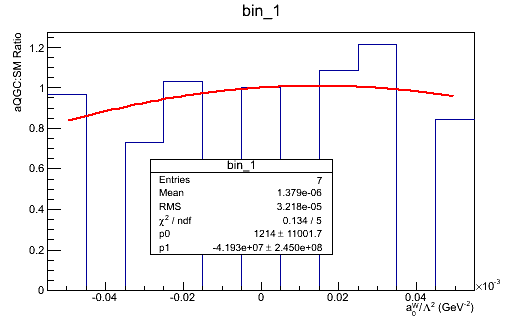
\includegraphics[width=0.33\textwidth]{figs/a0W_PhotonPT_para_bin1.png}
  }
    \subfigure[]{
    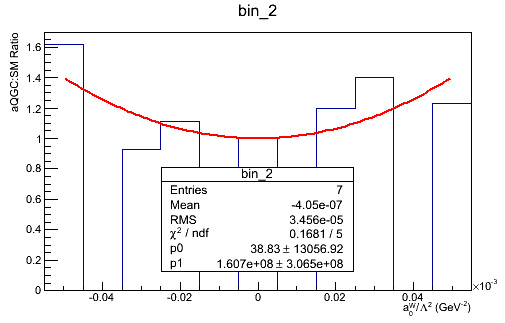
\includegraphics[width=0.33\textwidth]{figs/a0W_PhotonPT_para_bin2.png}
  }
    \subfigure[]{
    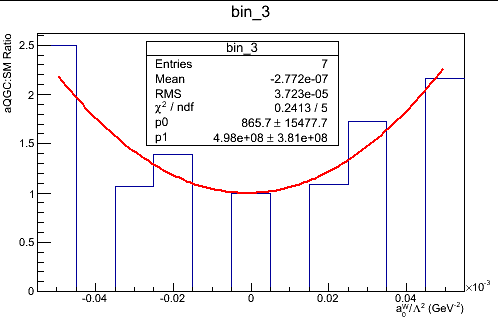
\includegraphics[width=0.33\textwidth]{figs/a0W_PhotonPT_para_bin3.png}
  }\\
    \subfigure[]{
    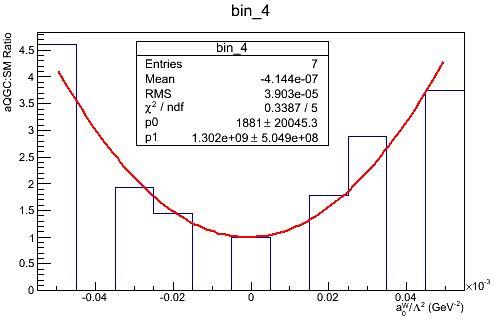
\includegraphics[width=0.33\textwidth]{figs/a0W_PhotonPT_para_bin4.png}
  }
    \subfigure[]{
    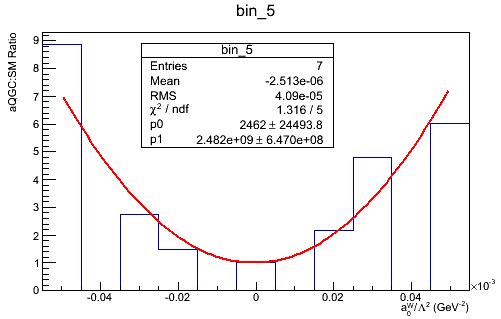
\includegraphics[width=0.33\textwidth]{figs/a0W_PhotonPT_para_bin5.png}
  }
    \subfigure[]{
    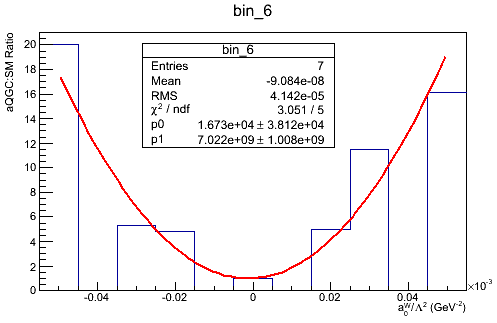
\includegraphics[width=0.33\textwidth]{figs/a0W_PhotonPT_para_bin6.png}
  }\\
    \subfigure[]{
    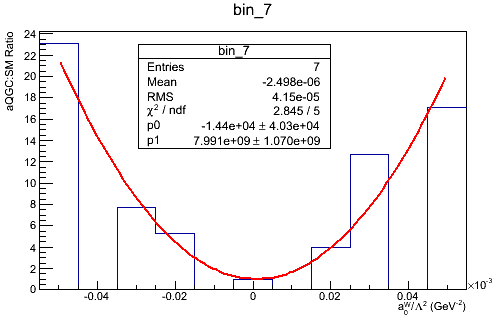
\includegraphics[width=0.33\textwidth]{figs/a0W_PhotonPT_para_bin7.png}
  }
    \subfigure[]{
    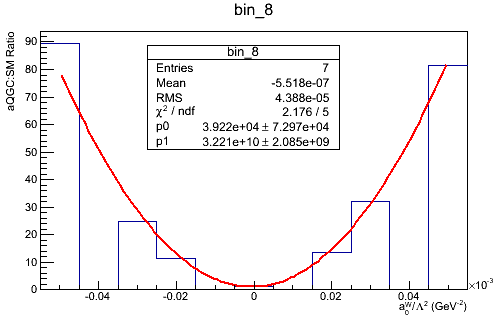
\includegraphics[width=0.33\textwidth]{figs/a0W_PhotonPT_para_bin8.png}
  }
    \subfigure[]{
    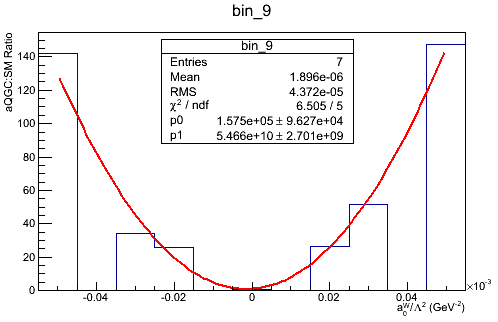
\includegraphics[width=0.33\textwidth]{figs/a0W_PhotonPT_para_bin9.png}
  }\\
    \subfigure[]{
    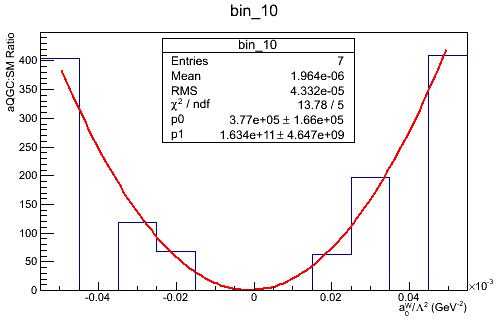
\includegraphics[width=0.33\textwidth]{figs/a0W_PhotonPT_para_bin10.png}
  }
    \caption{AQGC/SM ratio values for each $a_{0}^{W}/\Lambda^{2}$ Monte Carlo sample (muon channel) within each of the following Photon $p_{T}$ bins: Photon $p_{T}$ bins (a) 30-72 GeV, (b) 72-114 GeV, (c) 114-156 GeV, (d) 156-198 GeV, (e) 198-240 GeV, (f) 240-282 Gev, (g) 282-324 GeV, (h) 324-366 GeV, (i) 366-408 GeV, 408-inf. GeV (overflow bin)}
  \label{fig:para_ptbins}
  \end{center}
\end{figure}

We fit this quadratic distribution with a quadratic function that can later 
be used to predict the AQGC/SM ratio value for any arbitrary anomalous 
coupling value for that specific coupling parameter and photon $p_{T}$ bin. 
It can even been seen in Figure~\ref{fig:para_ptbins} that the overflow 
photon $p_{T}$ bin has a quadratic behavior in AQGC and thus can be 
parametrized.  

Keeping in mind that the AQGC/SM ratio fit function for a given coupling 
parameter is a function of the coupling parameter's value and depends on the
photon $p_{T}$ bin, we then plot and fit the coefficients of the AQGC/SM 
quadratic fit function versus photon $p_{T}$ in order to obtain the 
$p_T{}$-dependence of the AQGC/SM ratio.  Therefore, we obtain a 
parametrization of the affect each anomalous coupling parameter has on 
photon $p_{T}$ by substituting the $p_{T}$-dependent coefficient fit 
functions into the coupling parameter-dependent AQGC/SM ratio fit function, 
as shown in equation~\ref{parameq}.

\begin{center}
\begin{equation}
R(parameter,p_{T}) = \frac{\# AQGC events(parameter,p_{T})}{\# SM events(p_{T})} = 1 + C_{0}(p_{T}) \cdot parameter + C_{1}(p_{T}) \cdot parameter^{2}
\label{parameq}
\end{equation}
\end{center}

A closure test can be performed using equation~\ref{parameq} as a 
reweighting function applied to the Standard Model photon $p_{T}$ spectrum, 
as can be seen in Figure~\ref{fig:para_closure} for 
$\frac{a_{0}^{W}}{\Lambda^{2}}$ where the simulated (parametrized) Monte 
Carlo is compared to the generated (true) Monte Carlo.  Furthermore, the 
ratio between some of the simulated and generated Monte Carlo of each AQGC 
parameter can be seen in Figure~\ref{fig:para_closure_ratio}, where the 
deviation in each photon $p_{T}$ bin remains below 40\%.  The deviation in 
the overflow photon $p_{T}$ bin for each AQGC parameter remains below 15\% 
as well. A closure test ratio plot is also included in
Figure~\ref{fig:para_closure_ratio} for $\frac{a_{0}^{W}}{\Lambda^{2}}$ when using
a form factor of $\Lambda = 500 GeV, n = 2$.

\begin{figure}[]
  \begin{center}
    \subfigure[]{
    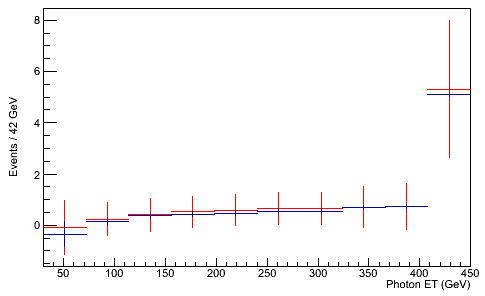
\includegraphics[width=0.45\textwidth]{figs/a0W_p5_closure.png}
  }
    \subfigure[]{
    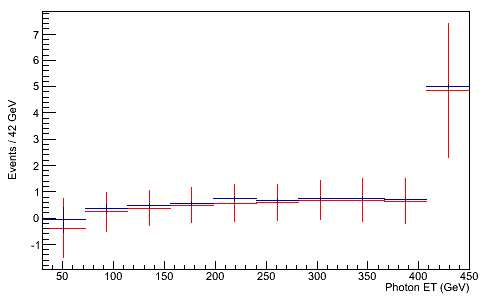
\includegraphics[width=0.45\textwidth]{figs/a0W_m5_closure.png}
  }
    \caption{Photon $p_{T}$ of simulated (Red line) and generated (Blue line) Monte Carlo samples for (a) $a_{0}^{W}/\Lambda^{2}$ = 5E-05 $GeV^{-2}$ and (b) $a_{0}^{W}/\Lambda^{2}$ = -5E-05 $GeV^{-2}$ (both are muon channel)}
  \label{fig:para_closure}
  \end{center}
\end{figure}

\begin{figure}[]
  \begin{center}
    \subfigure[]{
    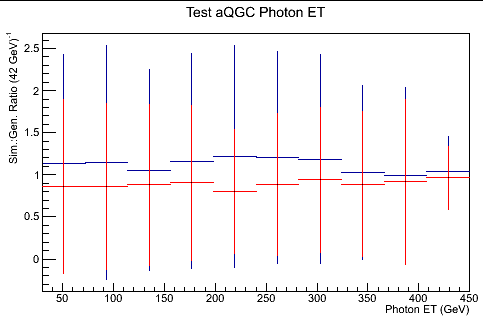
\includegraphics[width=0.45\textwidth]{figs/a0W_ratio.png}
  }
    \subfigure[]{
    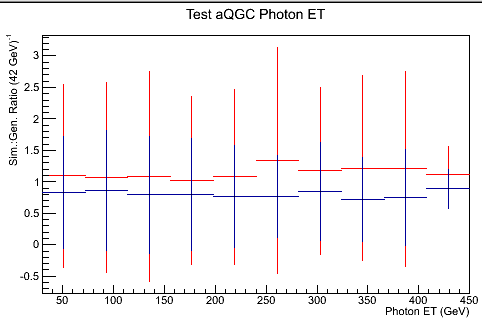
\includegraphics[width=0.45\textwidth]{figs/acW_ratio.png}
  }\\
    \subfigure[]{
    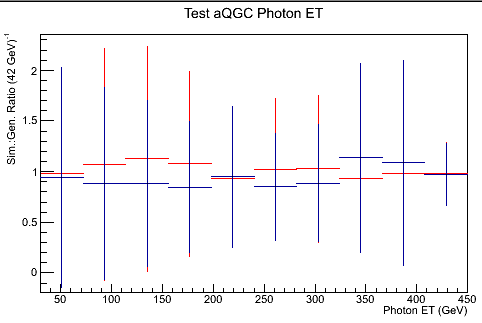
\includegraphics[width=0.45\textwidth]{figs/lt0_ratio.png}
  }
    \subfigure[]{
    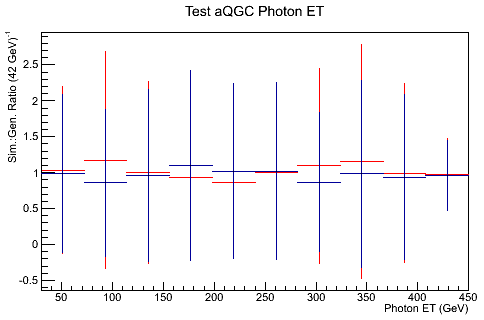
\includegraphics[width=0.45\textwidth]{figs/aQGC_K0W_closure_ratio.png}
  }\\
    \subfigure[]{
    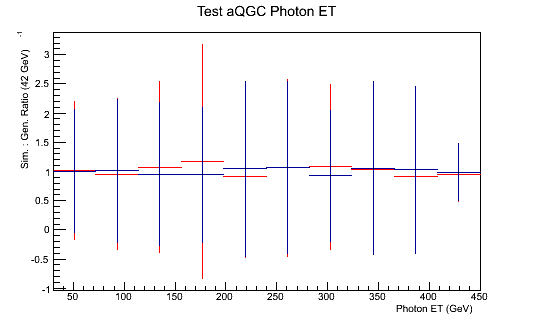
\includegraphics[width=0.45\textwidth]{figs/aQGC_KCW_closure_ratio.png}
  }
    \subfigure[]{
    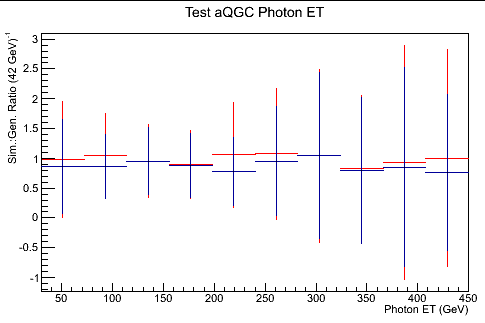
\includegraphics[width=0.45\textwidth]{figs/a0W_500FFn2_ratio.png}
  }
    \caption{Muon channel Simulated:Generated ratio as a function of photon $p_{T}$ for (a) $a_{0}^{W}/\Lambda^{2}$ = -5E-05 $GeV^{-2}$ (Red line), 5E-05 $GeV^{-2}$ (Blue line); (b) $a_{C}^{W}/\Lambda^{2}$ = -8E-05 $GeV^{-2}$ (Red line), 8E-05 $GeV^{-2}$ (Blue line); (c) $f_{T,0}/\Lambda^{4}$ = -8E-11 $GeV^{-2}$ (Red line), 8E-11 $GeV^{-2}$ (Blue line); (d) $\kappa_{0}^{W}/\Lambda^{2}$ = -2E-5 $GeV^{-2}$ (Red line), 2E-5 $GeV^{2}$ (Blue line); (e) $\kappa_{C}^{W}/\Lambda^{2}$ = -3E-5 $GeV^{-2}$ (Red line), 3E-5 $GeV^{2}$ (Blue line); (f) $a_{0}^{W}/\Lambda^{2}$ = -140E-05 $GeV^{-2}$ (Red line), 140E-05 $GeV^{-2}$ (Blue line) incorporating a Form Factor of $\Lambda = 500 GeV, n = 2$.}
  \label{fig:para_closure_ratio}
  \end{center}
\end{figure}

\newpage
\subsection{Limits using Photon $p_{T}$}
\label{sec:limits_pT}
We use the photon $p_T$ distribution as observable to set limit on anomalous
couplings.

We use the ``Higgs Combination'' package \cite{cite:combine} for
setting exclusion limits. This package is a
RooStats\cite{cite:roostats}-based statistical analysis tool-set
recommended by the CMS Higgs PAG and approved by CMS statistics committee.

We take as inputs the photon $p_T$ distributions for each signal model 
(\textit{i.e.}, various choices of $a_{0}^{W}/\Lambda^{2}$,  
$a_{C}^{W}/\Lambda^{2}$, $f_{T,0}/\Lambda^{4}$, $\kappa_{0}^{W}/\Lambda^{2}$, and 
$\kappa_{C}^{W}/\Lambda^{2}$), data, and total background that survive after
analysis cuts. All of these distributions are segregated by lepton flavor,
which represent independent channel inputs to the limit setter. 
Figure~\ref{fig:limitinput} shows the muon channel for given values of AQGC 
parameters, with and without MVA optimization (cut at 0.5), in which the AQGC input is the 
excess events from the SM prediction. For the MVA case in Figure~\ref{fig:limitinput},
the $f_{T,0}/\Lambda^{4}$ sample had diminished statistics after the cut on the MVA output
was made. We supply these distributions over the 
range $30-450~\GeV/c$ in the form of histograms to the limit setter. The binning 
is chosen such that the left-most bin begins at the first 2012 dataset point, and the 
right-most bin begins just beyond the last 2012 dataset point. We extend the
right-most bin to be an overflow bin, and since it begins just beyond the
reach of 2012 data in our events, it represents physics beyond our
sensitivity.

\begin{figure}[b]
  \begin{center}
    \subfigure[]{
      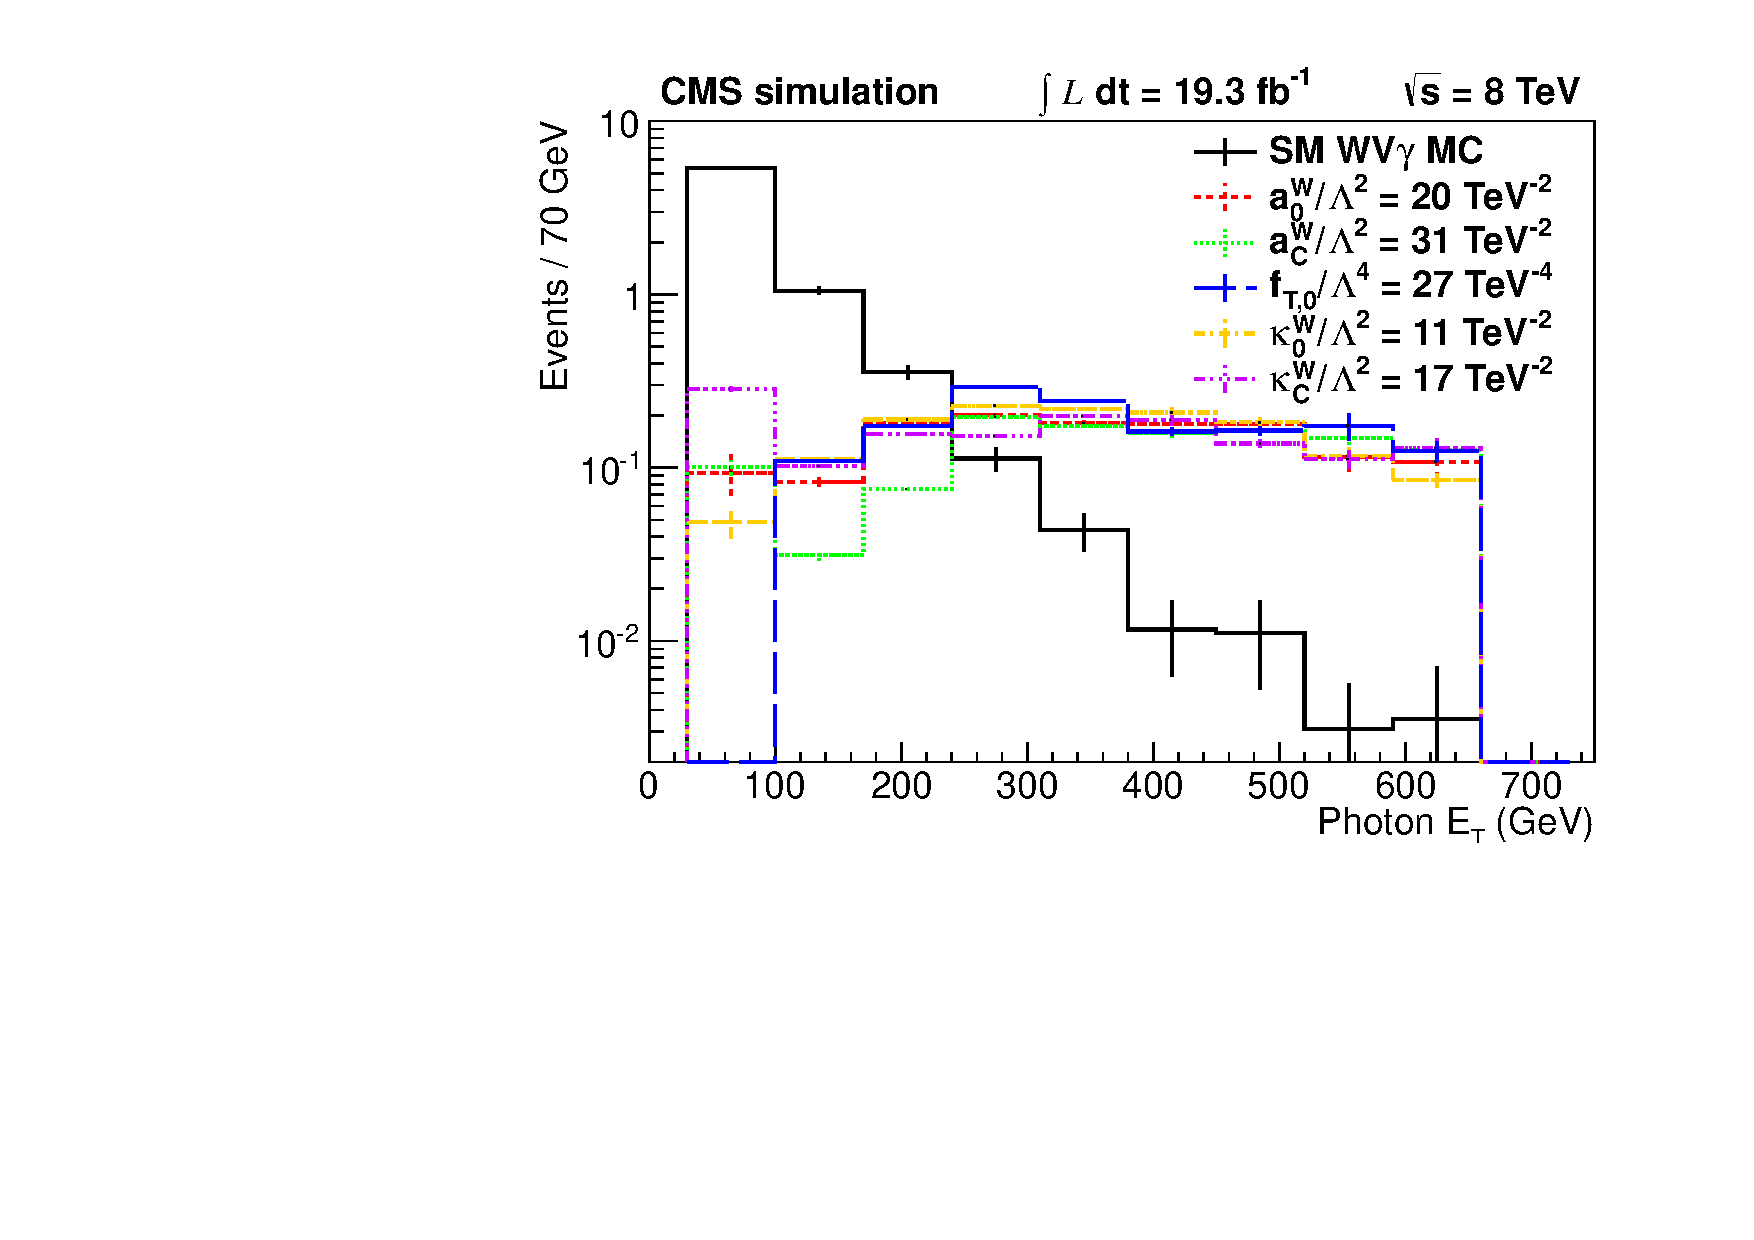
\includegraphics[width=0.45\textwidth]{figs/mu_limit_input.pdf}
    }
    \subfigure[]{
      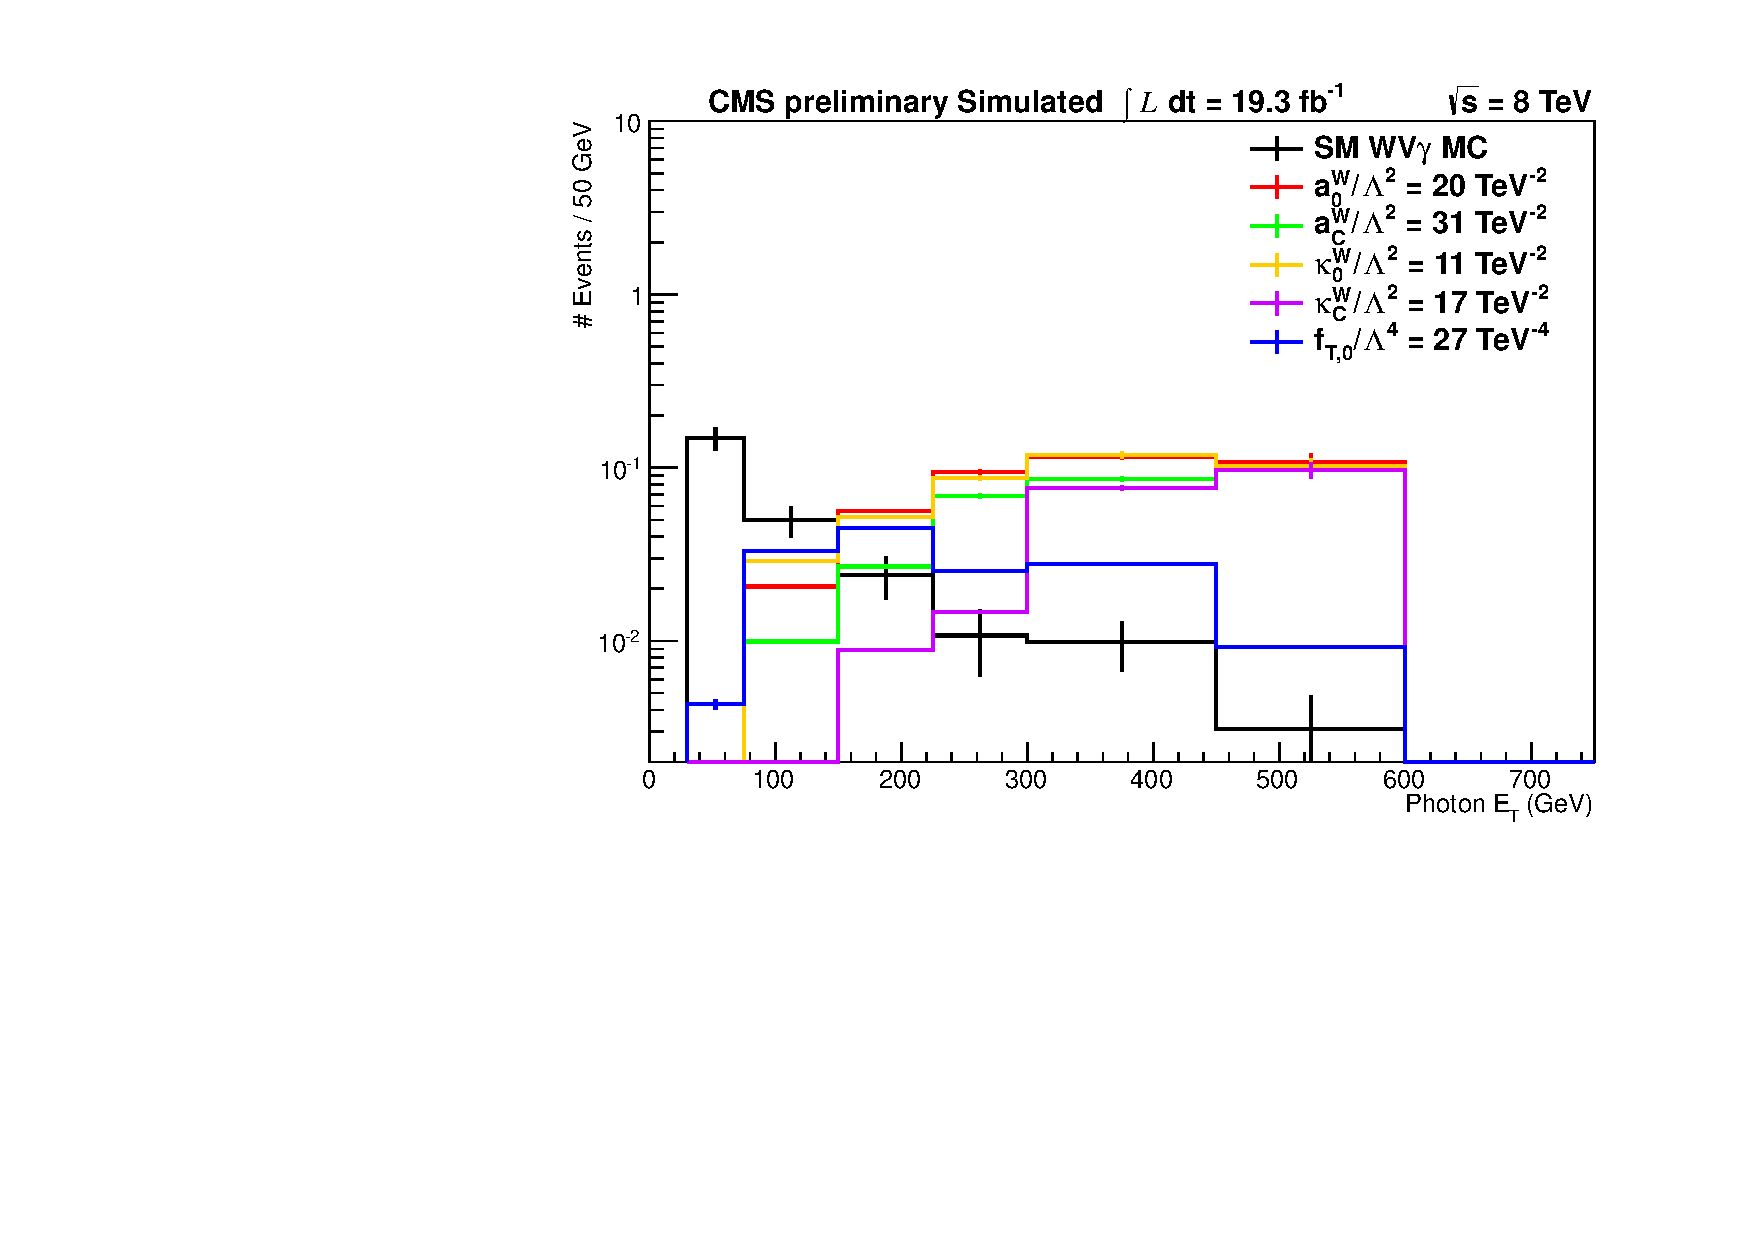
\includegraphics[width=0.45\textwidth]{figs/mu_limit_input_MVA.pdf}
    }
    \caption{ Input photon $p_{T}$ distributions for the limit setter of the muon channel (a) without MVA optimization and (b) with MVA optimization, cut at 0.5: SM prediction (Black); AQGC excess from SM prediction for $a_{0}^{W}/\Lambda^{2}$ (Red), $a_{C}^{W}/\Lambda^{2}$ (Green), $f_{T,0}/\Lambda^{4}$ (Blue), $\kappa_{0}^{W}/\Lambda^{2}$ (Orange), and $\kappa_{C}^{W}/\Lambda^{2}$ (Violet). }
    \label{fig:limitinput}
  \end{center}
\end{figure}

The limit setter is then set to utilize the ``ProfileLikelihood CL$_{s}$''
\cite{cite:asympcls1,cite:asympcls2} method. Figure~\ref{fig:limitshape1d_noMVA} 
is the resulting shape-based observed 
and expected exclusion limits without MVA optimization discussed in 
Section~\ref{sec:MVA}.  Exclusion limits for $a_{0}^{W}/\Lambda^{2}$, 
$a_{C}^{W}/\Lambda^{2}$, $f_{T,0}/\Lambda^{4}$, $\kappa_{0}^{W}/\Lambda^{2}$, and 
$\kappa_{C}^{W}/\Lambda^{2}$ are computed at the 95\% CL and are listed in
Table~\ref{tab:limit_values_noMVA} for the analysis without MVA optimization
discussed in Section~\ref{sec:MVA}. Table~\ref{tab:limit_values_noMVA_dim8}
contains the transformed Dimension 8 limits from the Dimension 6 a$_{0}^{W}$
and a$_{C}^{W}$ parameters, without MVA optimization. 

\begin{table}[htb]
\centering
\scalebox{1.0}{
  \begin{tabular}{|c|c|}
  \hline
  Observed Limits & Expected Limits \\
  \hline
  \hline
  -21 ($TeV^{-2}$) $<$ $a_{0}^{W}/\Lambda^{2}$ $<$ 20 ($TeV^{-2}$)  & -24 ($TeV^{-2}$) $<$ $a_{0}^{W}/\Lambda^{2}$ $<$ 23 ($TeV^{-2}$) \\
  -34 ($TeV^{-2}$) $<$ $a_{C}^{W}/\Lambda^{2}$ $<$ 32 ($TeV^{-2}$)  & -37 ($TeV^{-2}$) $<$ $a_{C}^{W}/\Lambda^{2}$ $<$ 34 ($TeV^{-2}$) \\
  -25 ($TeV^{-4}$) $<$ $f_{T,0}/\Lambda^{4}$ $<$ 24 ($TeV^{-4}$)  & -27 ($TeV^{-4}$) $<$ $f_{T,0}/\Lambda^{4}$ $<$ 27 ($TeV^{-4}$) \\
  -12 ($TeV^{-2}$) $<$ $\kappa_{0}^{W}/\Lambda^{2}$ $<$ 10 ($TeV^{-2}$)  & -12 ($TeV^{-2}$) $<$ $\kappa_{0}^{W}/\Lambda^{2}$ $<$ 12 ($TeV^{-2}$) \\
  -18 ($TeV^{-2}$) $<$ $\kappa_{C}^{W}/\Lambda^{2}$ $<$ 17 ($TeV^{-2}$)  & -19 ($TeV^{-2}$) $<$ $\kappa_{C}^{W}/\Lambda^{2}$ $<$ 18 ($TeV^{-2}$) \\
  \hline
  \end{tabular}}
  \caption{95\% CL shape-based exclusion limits listed for both the muon and electron channels of each AQGC parameter without MVA optimization, using photon $p_{T}$.}
  \label{tab:limit_values_noMVA}
\end{table}

\begin{table}[htb]
\centering
  \scalebox{1.0}{
  \begin{tabular}{|c|c|}
  \hline
  Observed Limits & Expected Limits \\
  \hline
  \hline
  -77 (TeV$^{-4}$) $<$ $f_{M,0}/\Lambda^{4}$ $<$ 81 (TeV$^{-4}$)  & -89 (TeV$^{-4}$) $<$ $f_{M,0}/\Lambda^{4}$ $<$ 93 (TeV$^{-4}$) \\
  -131 (TeV$^{-4}$) $<$ $f_{M,1}/\Lambda^{4}$ $<$ 123 (TeV$^{-4}$)    & -143  (TeV$^{-4}$) $<$ $f_{M,1}/\Lambda^{4}$ $<$ 131  (TeV$^{-4}$) \\
  -39 (TeV$^{-4}$) $<$ $f_{M,2}/\Lambda^{4}$ $<$ 40 (TeV$^{-4}$)  & -44 (TeV$^{-4}$) $<$ $f_{M,2}/\Lambda^{4}$ $<$ 46 (TeV$^{-4}$) \\
  -66 (TeV$^{-4}$) $<$ $f_{M,3}/\Lambda^{4}$ $<$ 62 (TeV$^{-4}$)    & -71  (TeV$^{-4}$) $<$ $f_{M,3}/\Lambda^{4}$ $<$ 66  (TeV$^{-4}$) \\
  \hline
  \end{tabular}}  \caption{95\% CL shape-based exclusion limits listed for both the muon and electron channels of each Dim. 8 AQGC parameter without MVA optimization, using photon $p_{T}$.}
  \label{tab:limit_values_noMVA_dim8}
\end{table}


\begin{figure}[hb]
  \begin{center}
    \subfigure[]{
    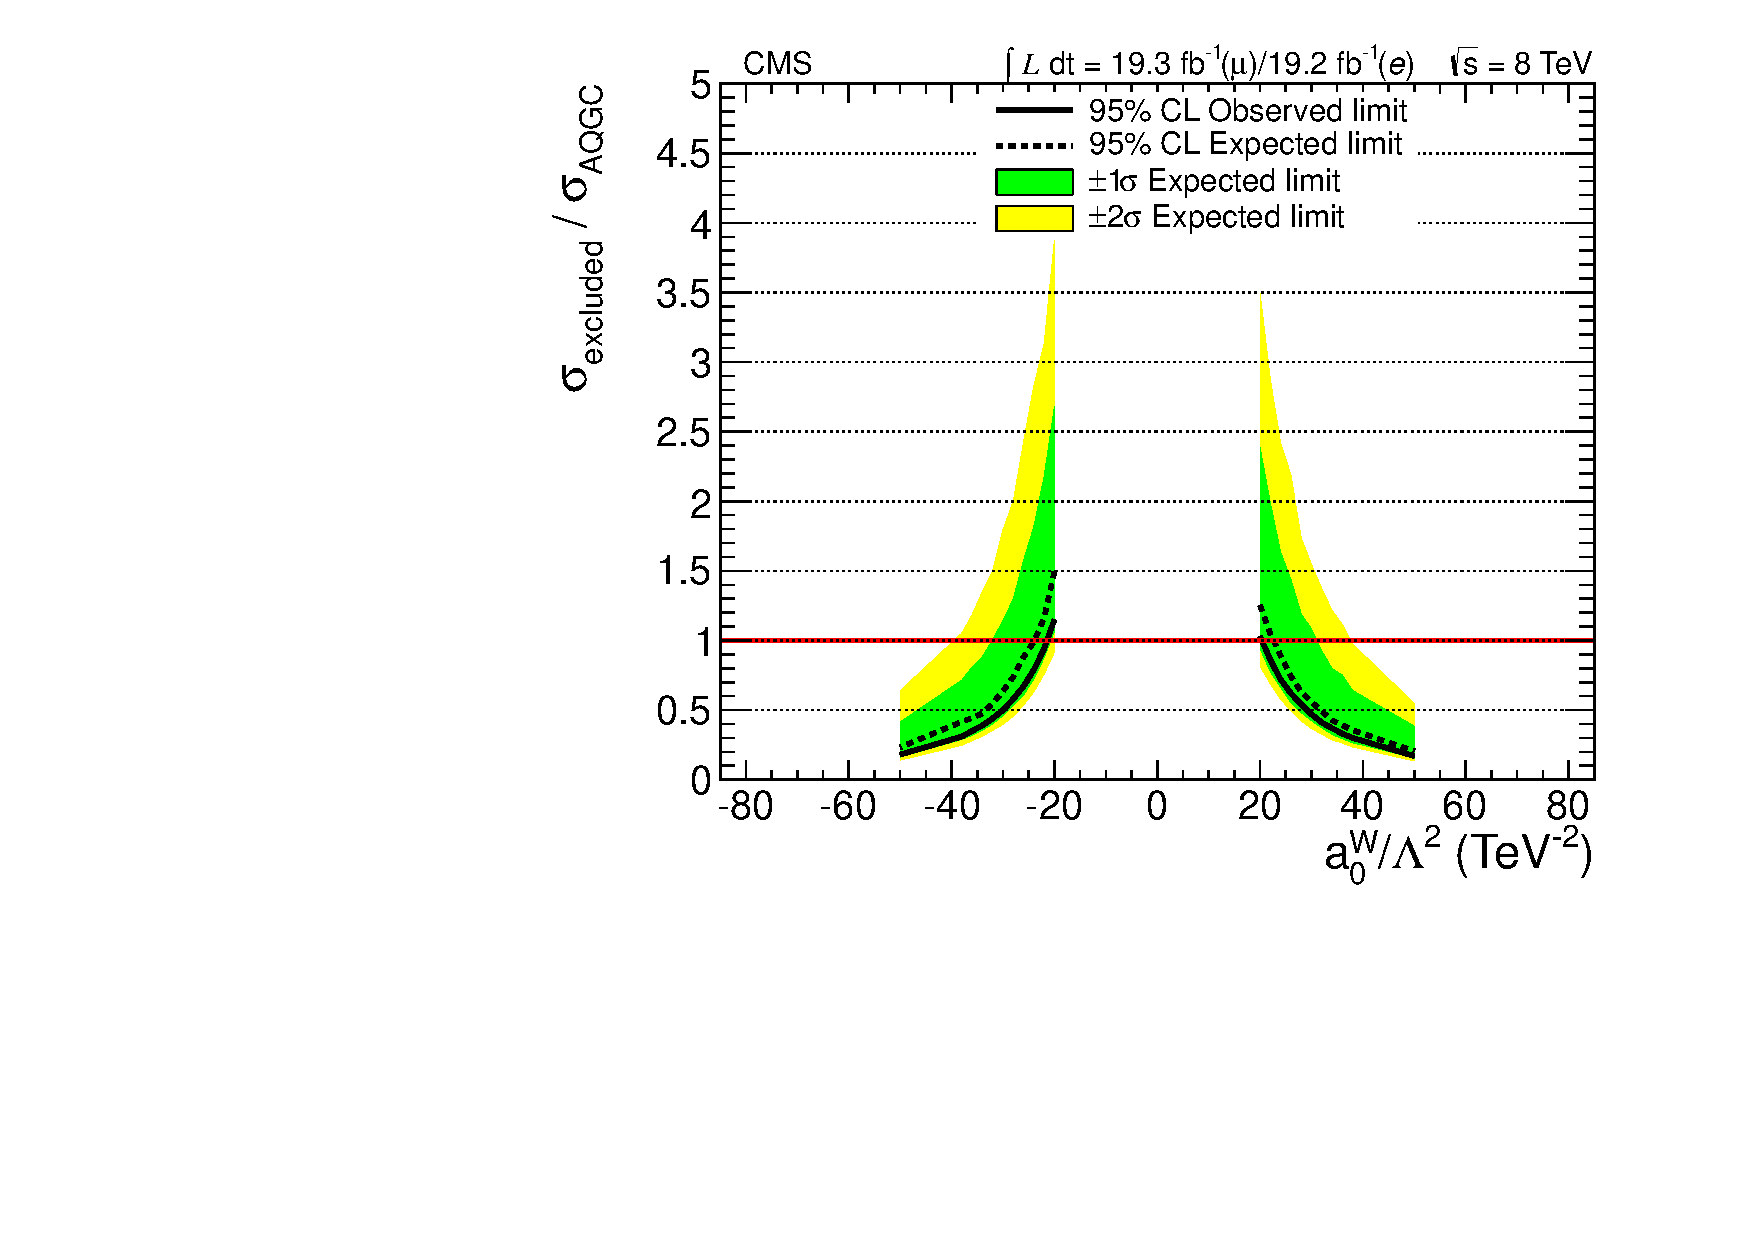
\includegraphics[width=0.45\textwidth]{figs/a0W_PhotonPT_limit_noMVA.pdf}
  }
    \subfigure[]{
    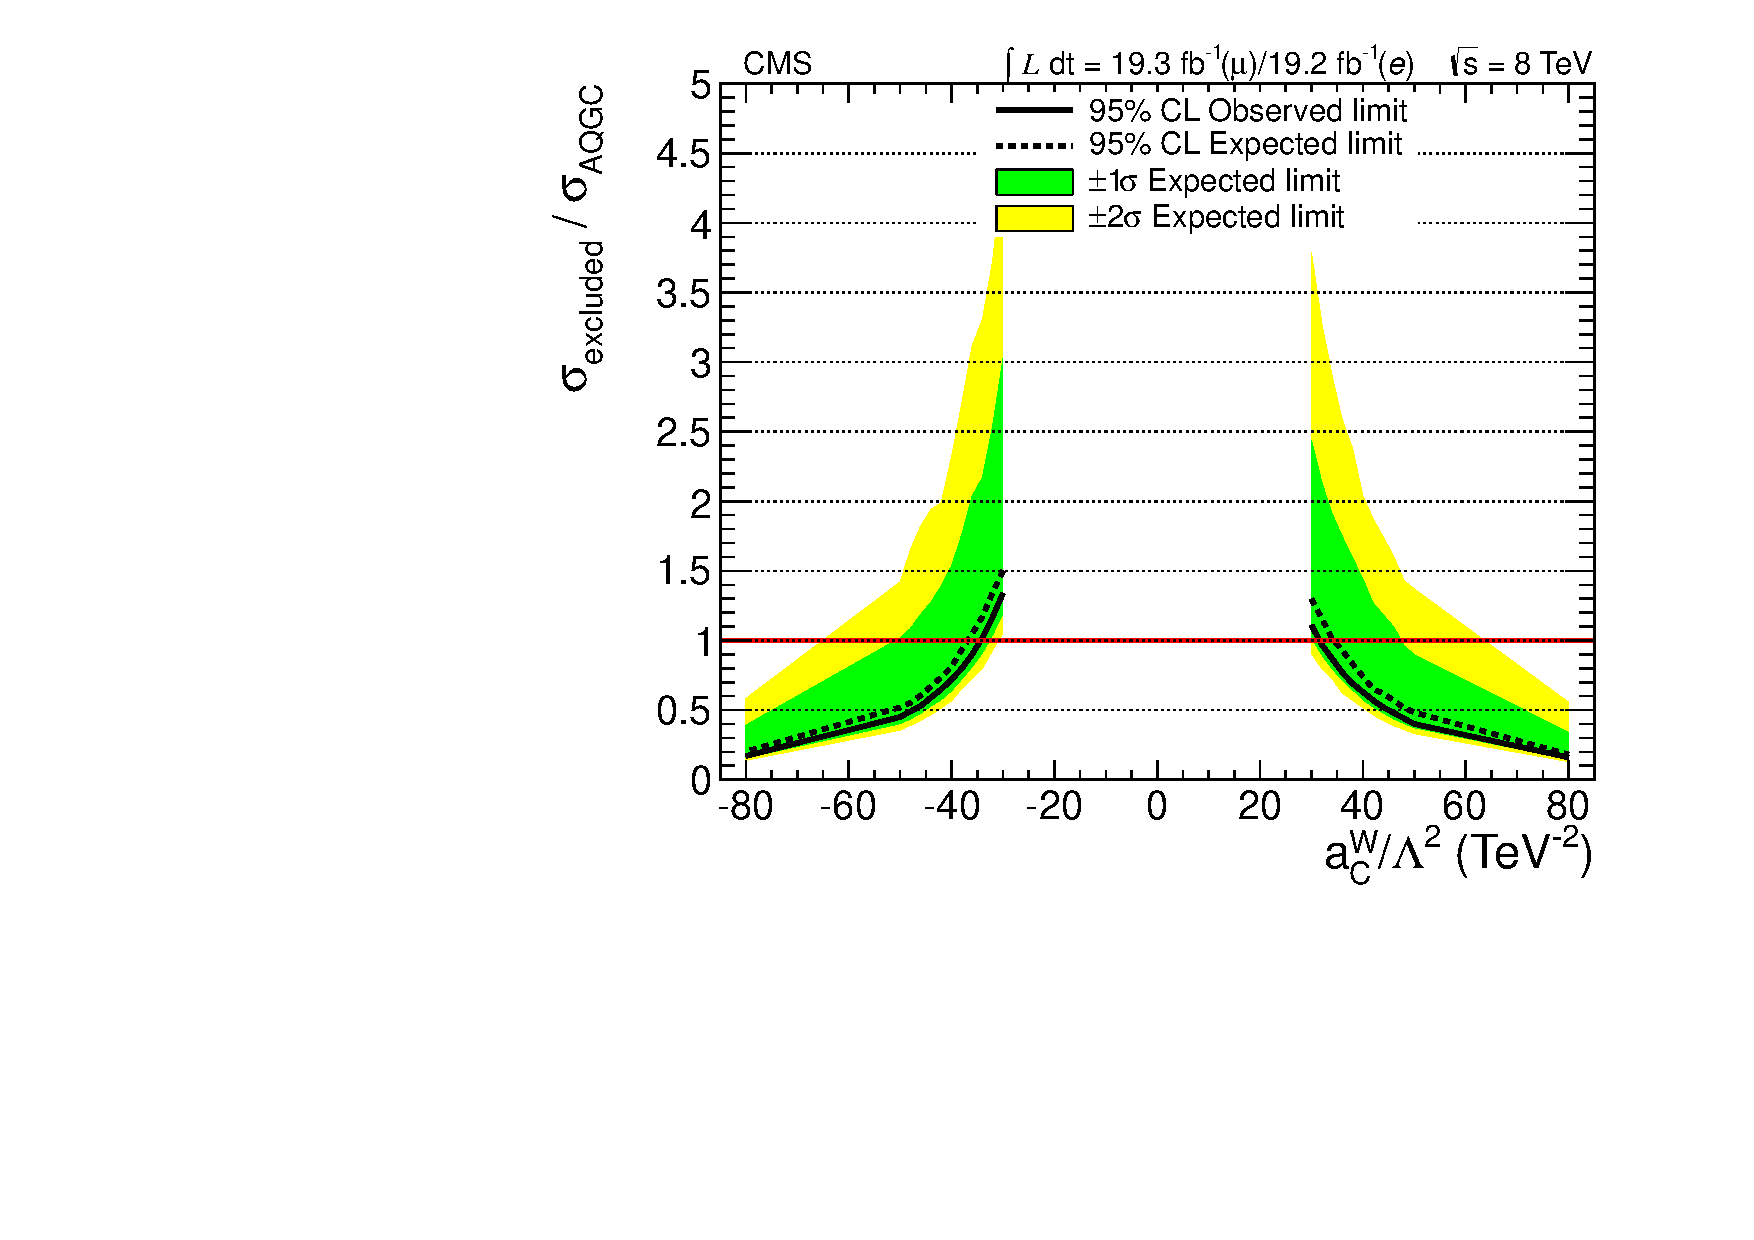
\includegraphics[width=0.45\textwidth]{figs/acW_PhotonPT_limit_noMVA.pdf}
  }\\
  \subfigure[]{
    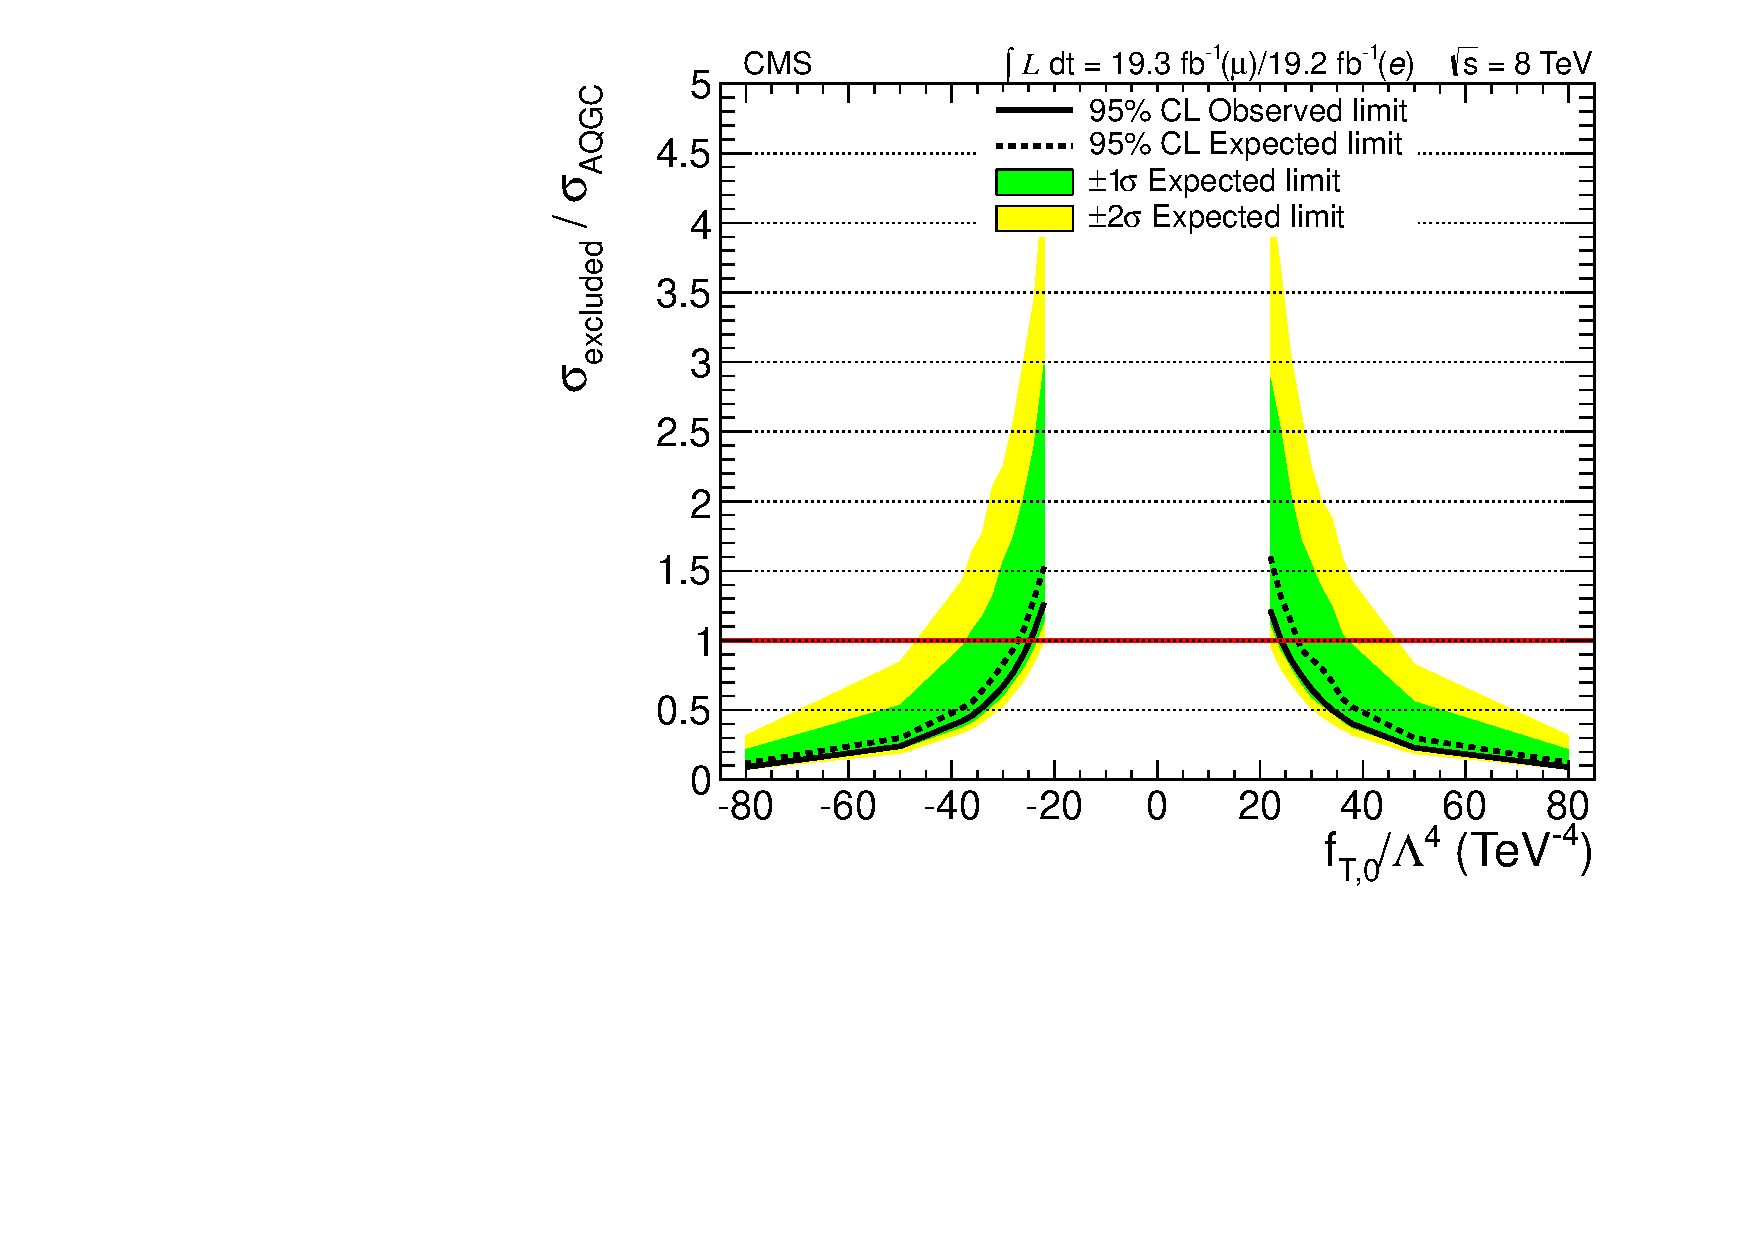
\includegraphics[width=0.45\textwidth]{figs/LT0_PhotonPT_limit_noMVA.pdf}
  }
  \subfigure[]{
    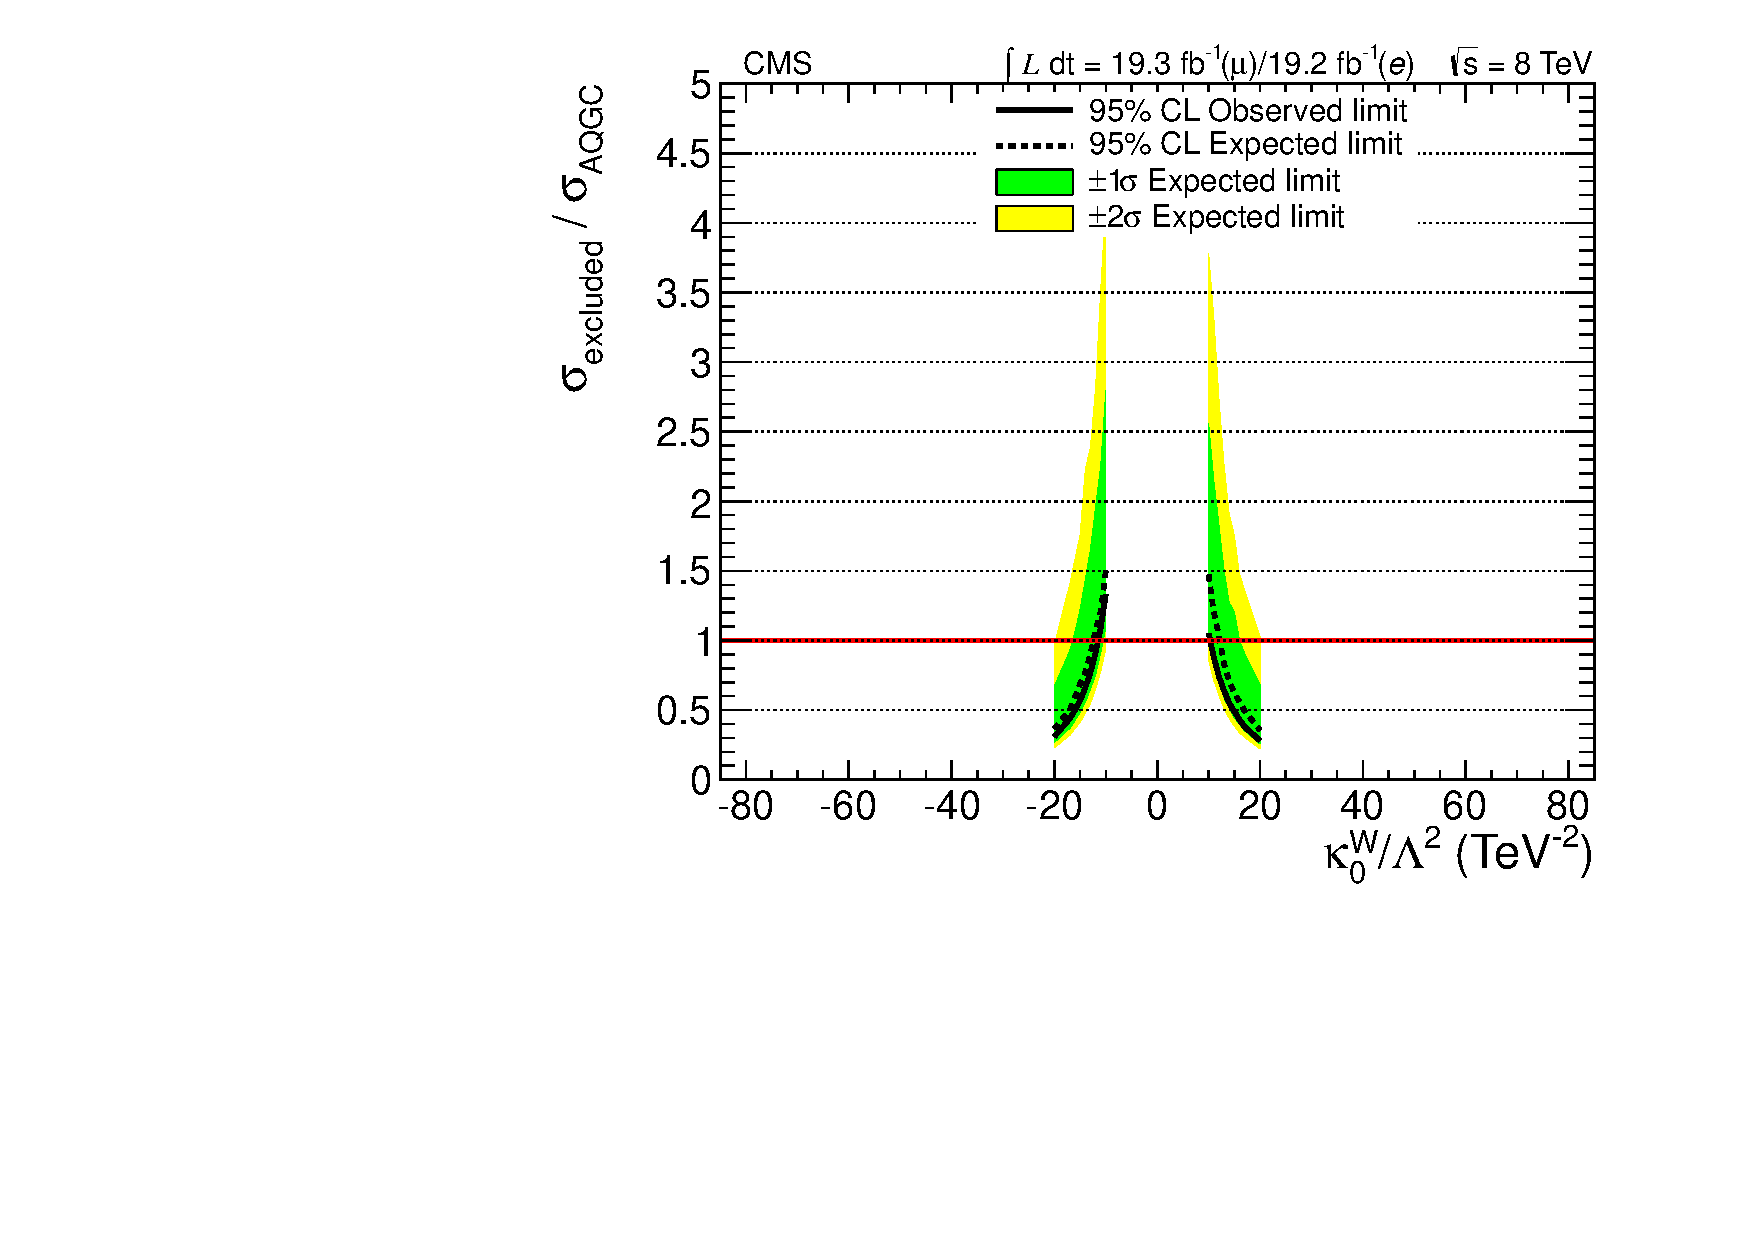
\includegraphics[width=0.45\textwidth]{figs/K0W_PhotonPT_limit_noMVA.pdf}
  }\\
  \subfigure[]{
    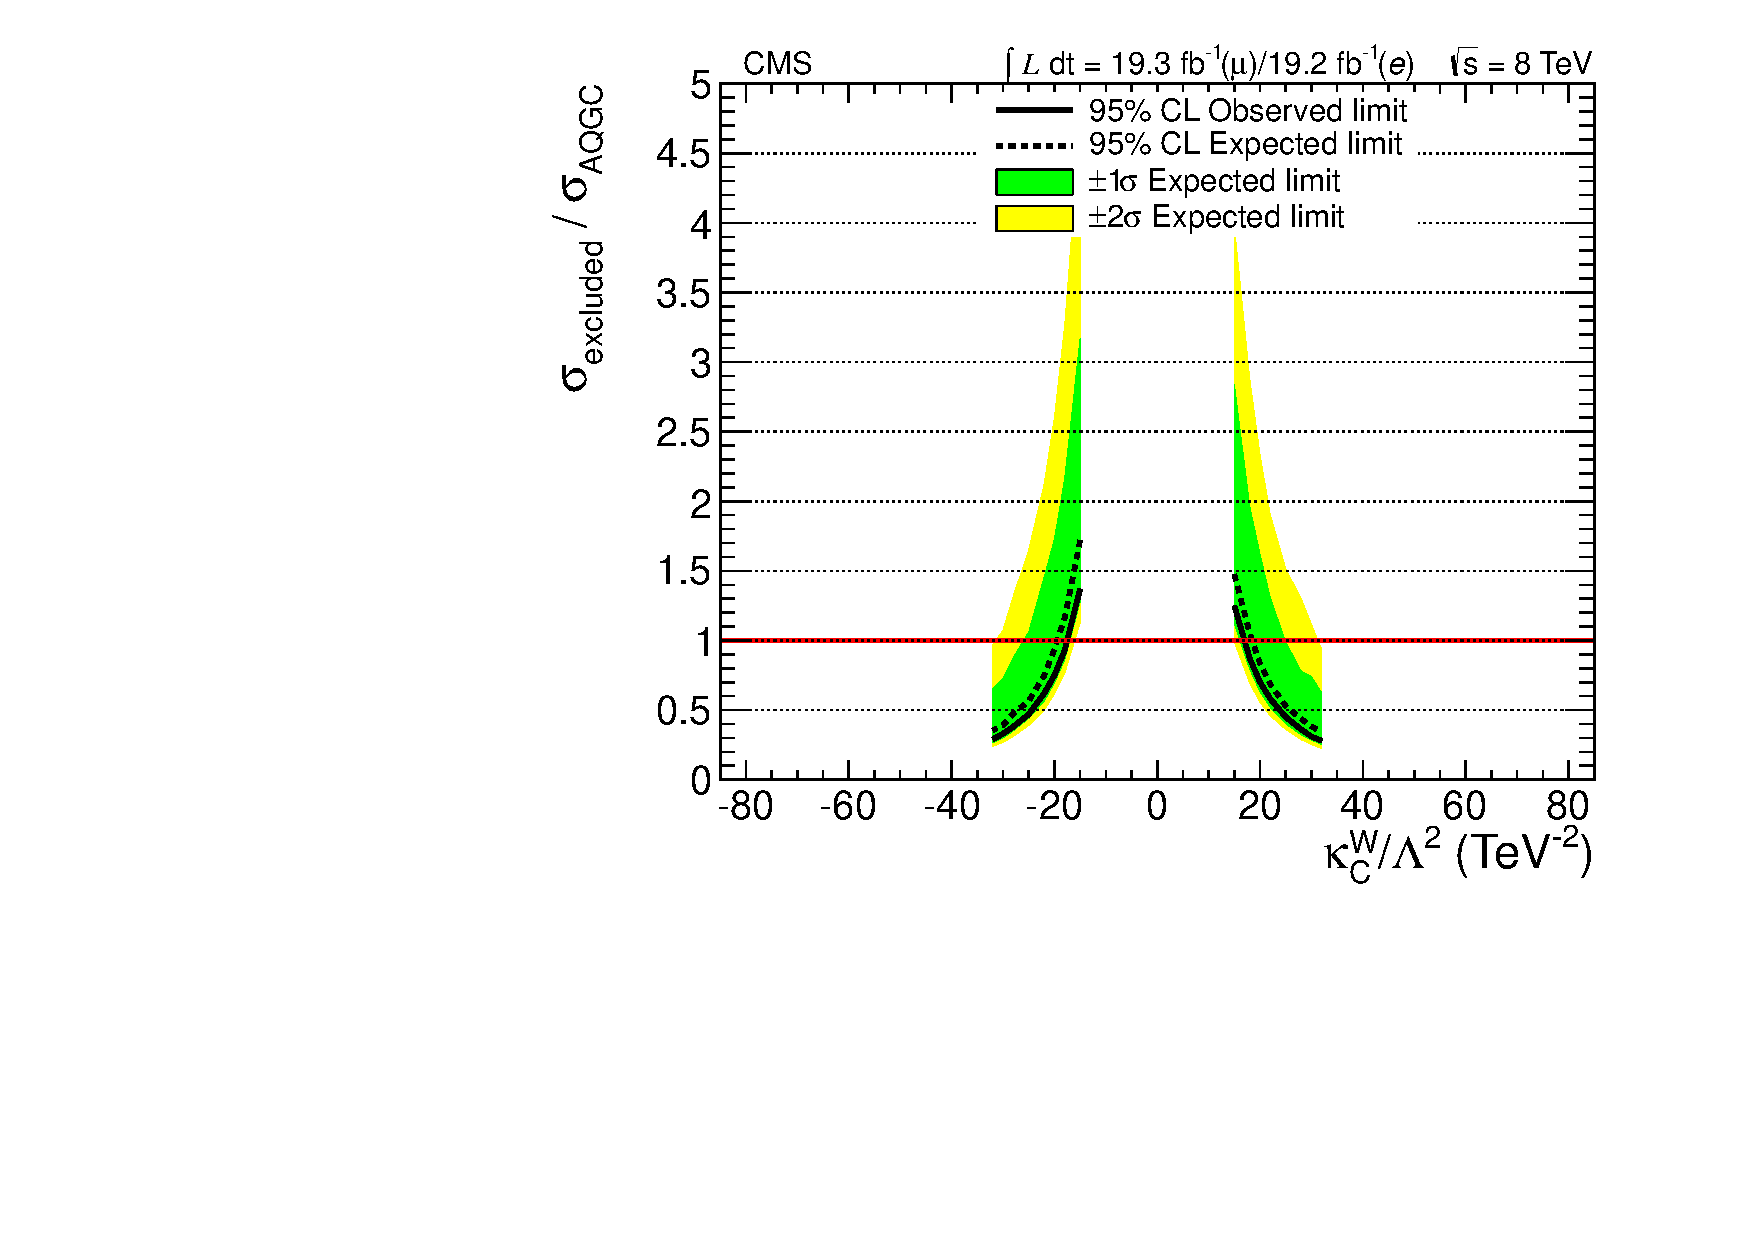
\includegraphics[width=0.45\textwidth]{figs/KCW_PhotonPT_limit_noMVA.pdf}
  }
  \subfigure[]{
    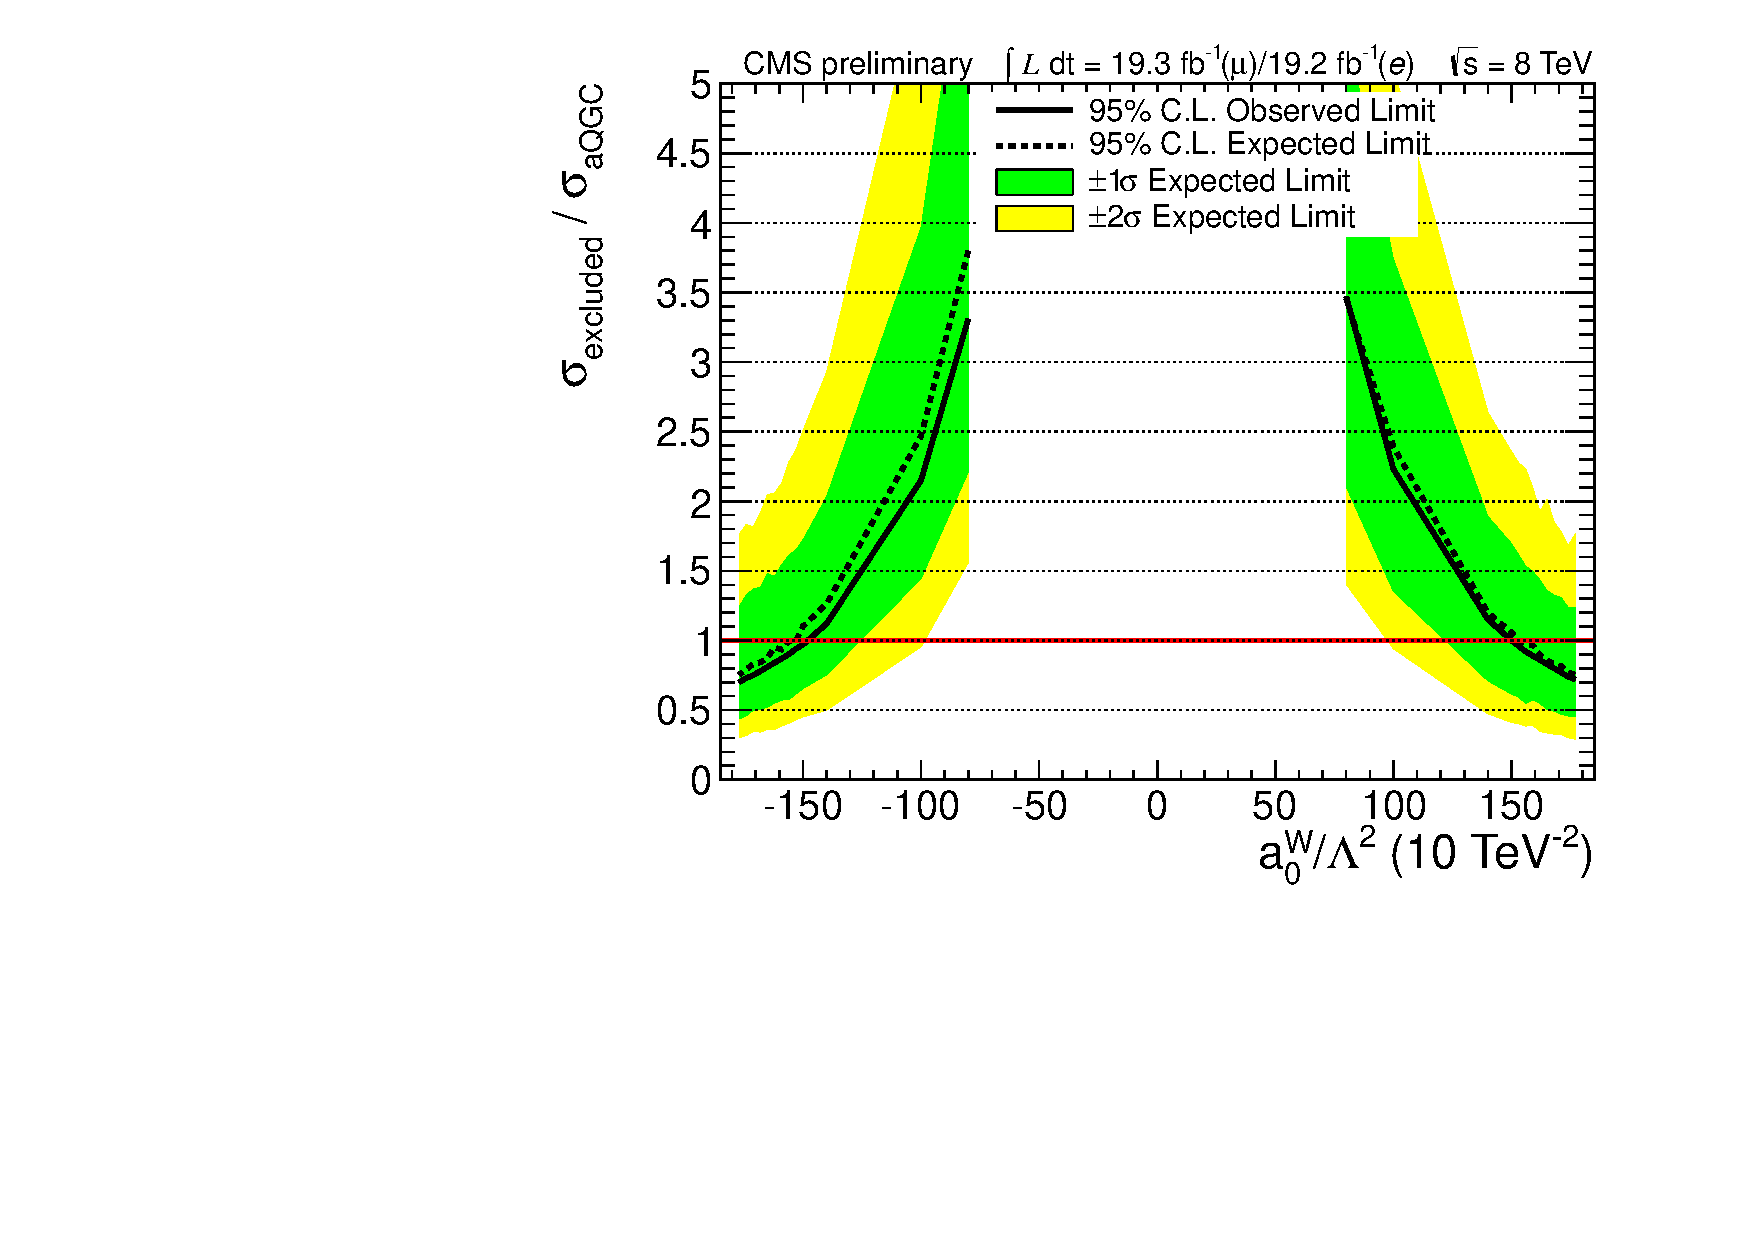
\includegraphics[width=0.45\textwidth]{figs/a0W_PhotonPT_limit_noMVA_500FFn2.pdf}
  }
    \caption{ Exclusion limits for (a) $a_{0}^{W}/\Lambda^{2}$; (b) $a_{C}^{W}/\Lambda^{2}$; (c) $f_{T,0}/\Lambda^{4}$; (d) $\kappa_{0}^{W}/\Lambda^{2}$; (e) $\kappa_{C}^{W}/\Lambda^{2}$; (f) $a_{0}^{W}/\Lambda^{2}$ with Form Factor $\Lambda = 500 GeV, n = 2$, all at the 95\% CL and no MVA optimization, using photon $p_{T}$.}
    \label{fig:limitshape1d_noMVA}
  \end{center}
\end{figure}


\subsection{Limits using M$_{WW\gamma}$}
\label{sec:limits_Mlvjja}
As an additional means of setting limits on AQGC, we performed the same
limit setting procedure previously discussed while using the WW$\gamma$
invariant mass as the descriminating distribution. Much like the photon
$p_{T}$ distribution, the $M_{WW\gamma}$ distribution experiences an
increase in the tail end of its spectrum (high-mass region) as a result of
AQGC; however, this distribution experiences much desctructive interefence
in the low mass region ($< 700 GeV/c^{2}$). We obtain a parametrization of 
AQGC as a function of the $a_{0}^{W}/\Lambda^{2}$ parameter
and WW$\gamma$ invariant mass, and Figure~\ref{fig:limits_Mlvjja} shows the 
resulting limits. Table~\ref{tab:limit_values_Mlvjja} lists the observed and expected limits at 
95\% CL We did not perform
MVA optimization in obtaining these limits, as our sensitivity was not
significantly increased by MVA methods (see Section~\ref{sec:limits_MVA}).
The behavior of the observed limits and the existence of destructive
interference makes this distribution not as optimal as photon $p_{T}$.

\begin{table}[htb]
\centering
\scalebox{1.0}{
  \begin{tabular}{|c|c|}
  \hline
  Observed Limits & Expected Limits \\
  \hline
  \hline
  -19 ($TeV^{-2}$) $<$ $a_{0}^{W}/\Lambda^{2}$ $<$ 16 ($TeV^{-2}$)  & -31 ($TeV^{-2}$) $<$ $a_{0}^{W}/\Lambda^{2}$ $<$ 28 ($TeV^{-2}$) \\
  \hline
  \end{tabular}}
  \caption{95\% CL shape-based exclusion limits listed for both the muon and electron channels of the AQGC parameter $a_{0}^{W}/\Lambda^{2}$, using $M_{WW\gamma}$ and without MVA optimization.}
  \label{tab:limit_values_Mlvjja}
\end{table}

\begin{figure}[hb]
  \begin{center}
    \subfigure[]{
    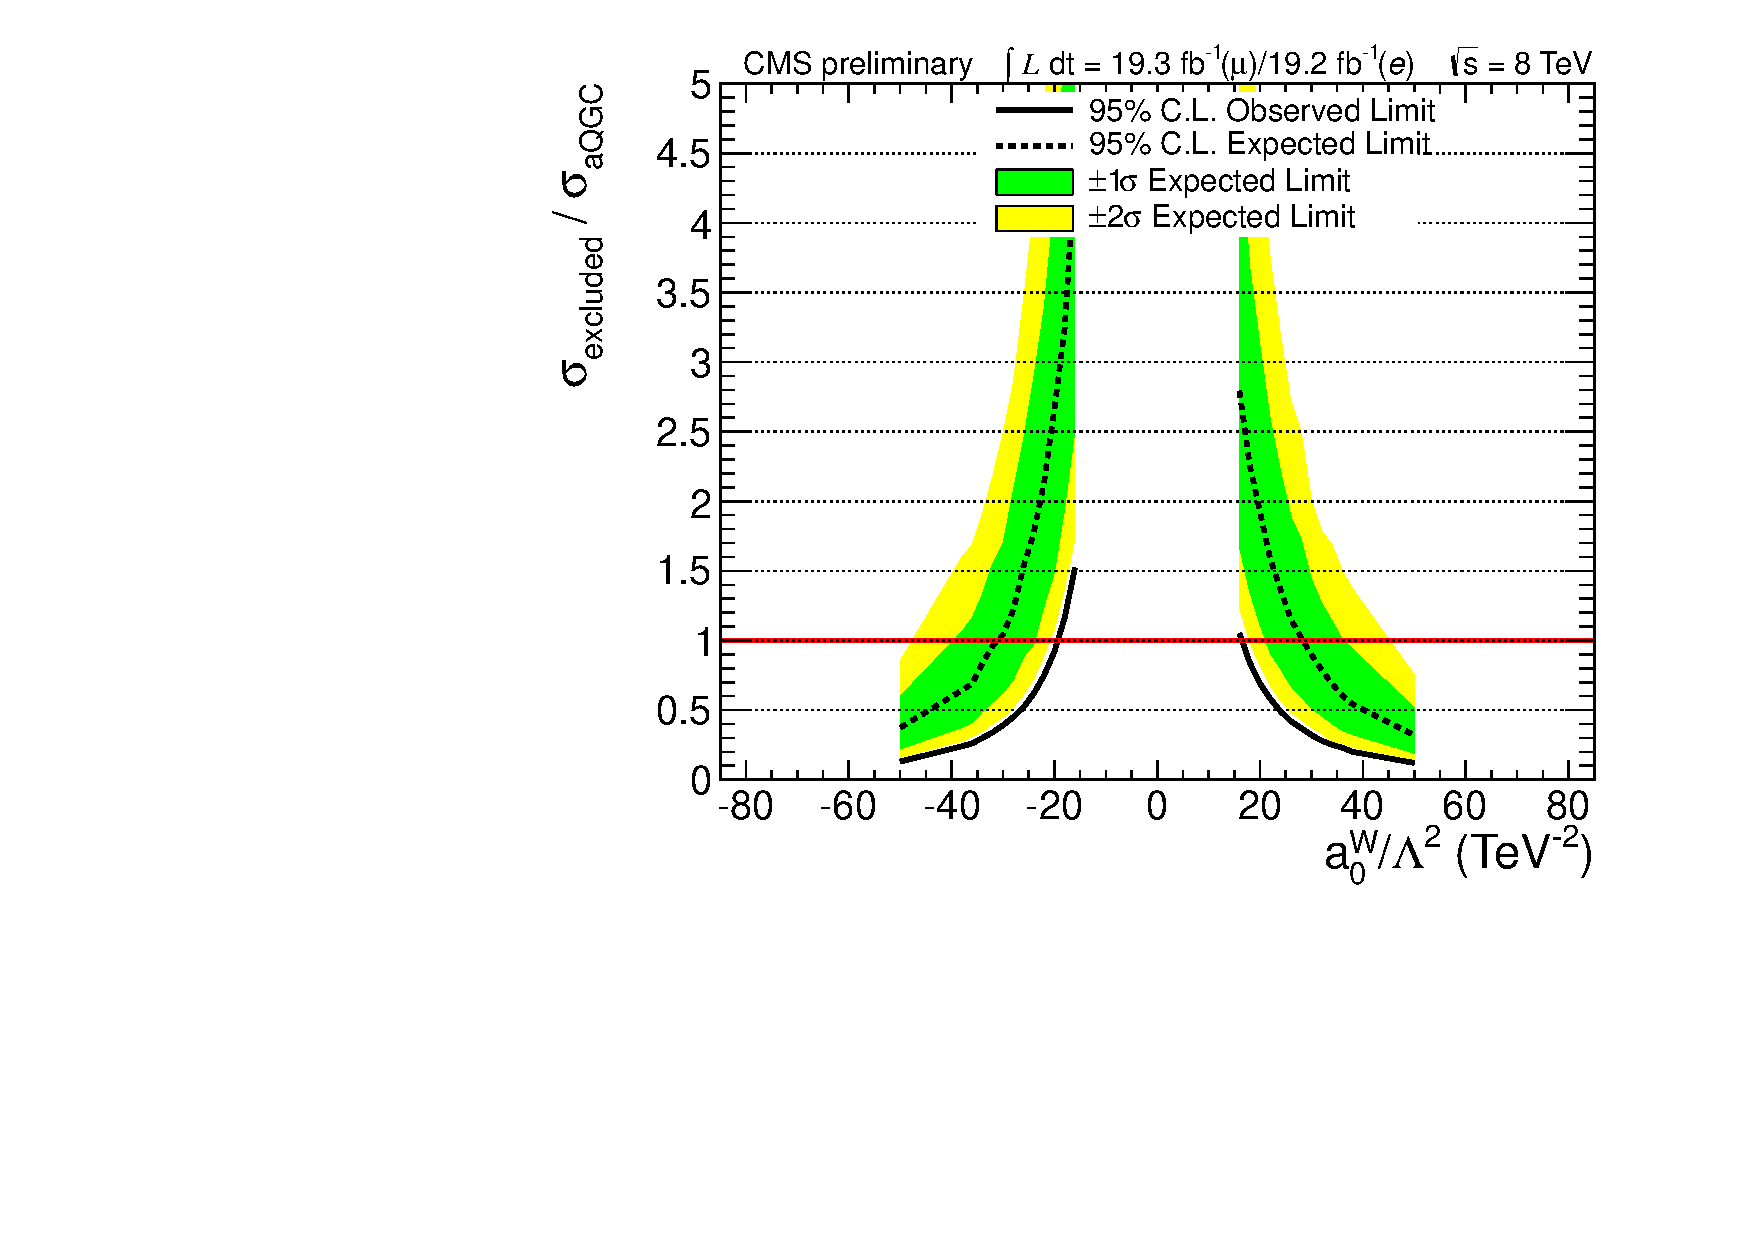
\includegraphics[width=0.45\textwidth]{figs/a0W_Mlvjja_limit_noMVA.pdf}
  }
    \caption{ Exclusion limits for $a_{0}^{W}/\Lambda^{2}$ at 95\% CL and no MVA optimization, using M$_{WW\gamma}$.}
    \label{fig:limits_Mlvjja}
  \end{center}
\end{figure}

\subsection{$a_{0}^{W}$ Limits using MVA}
\label{sec:limits_MVA}
In order to demonstrate the effect of MVA optimization on extracted limits
for one of our parameters, $a_{0}^{W}$, we varied the MVA cut value and
produced the limits shown in Figure~\ref{fig:limits_MVA} and 
Figure~\ref{fig:limits_MVA_FF}. It is shown that
MVA optimization does not improve the extracted limits beyond the original
sigma bands shown in Figure~\ref{fig:limitshape1d_noMVA}. Only the expected
limit is shown to demonstrate the best limits we could achieve. 
Table~\ref{tab:limit_values_MVA} lists the best expected limits from the MVA 
cut scan for the non-Form Factor limits at a MVA cut value of 0.5. 
The minor improvement in the limit do not justify the use of MVA techniques, thus we consider as a primary result the limits without MVA selection optimization.
%Table~\ref{tab:limit_values_MVA_FF} lists the best expected limits from the MVA cut scan for the 
%Form Factor limits at a MVA cut value of 0.1.

\begin{table}[htb]
\centering
\scalebox{1.0}{
  \begin{tabular}{|c|}
  \hline
  Expected Limits \\
  \hline
  \hline
  -24 ($TeV^{-2}$) $<$ $a_{0}^{W}/\Lambda^{2}$ $<$ 21 ($TeV^{-2}$)\\
  \hline
  \end{tabular}}
  \caption{95\% CL shape-based expected limits listed for both the muon and electron channels of the AQGC parameter $a_{0}^{W}/\Lambda^{2}$, using Photon $p_{T}$ and with MVA optimization cut = 0.5.}
  \label{tab:limit_values_MVA}
\end{table}

%\begin{table}[htb]
%\centering
%\scalebox{0.70}{
%  \begin{tabular}{|c|}
%  \hline
%  Expected Limits \\
%  \hline
%  \hline
%  -151 (10 $TeV^{-2}$) $<$ $a_{0}^{W}/\Lambda^{2}$ $<$ 149 (10 $TeV^{-2}$)\\
%  \hline
%  \end{tabular}}
%  \caption{95\% C.L. shape-based expected limits listed for both the muon and electron channels of the aQGC parameter $a_{0}^{W}/\Lambda^{2}$, Form Factor $\Lambda = 500 GeV, n = 2$, using Photon $p_{T}$ and with MVA optimization cut = 0.1.}
%  \label{tab:limit_values_MVA_FF}
%\end{table}

\begin{figure}[hb]
  \begin{center}
    \subfigure[]{
    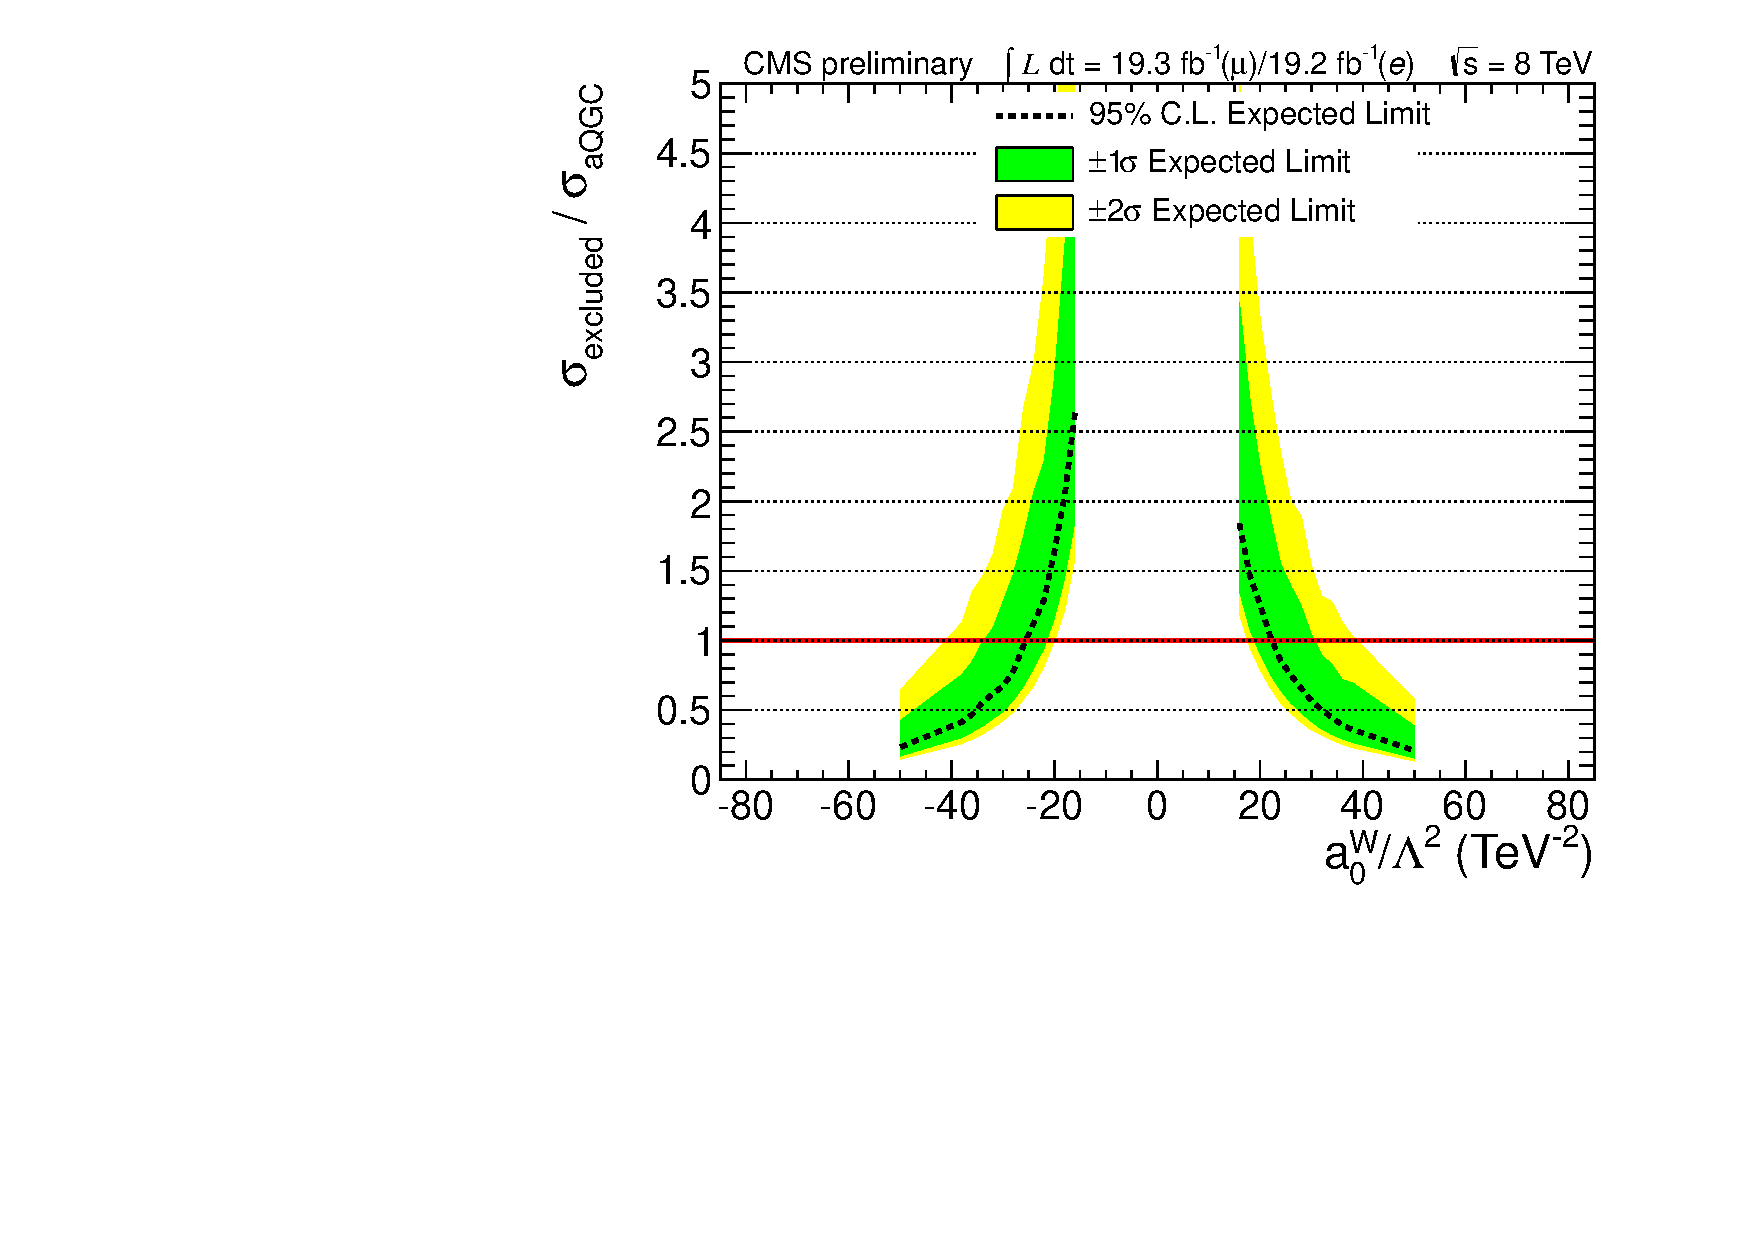
\includegraphics[width=0.33\textwidth]{figs/a0W_PhotonPT_limit_MVA01.pdf}
  }
    \subfigure[]{
    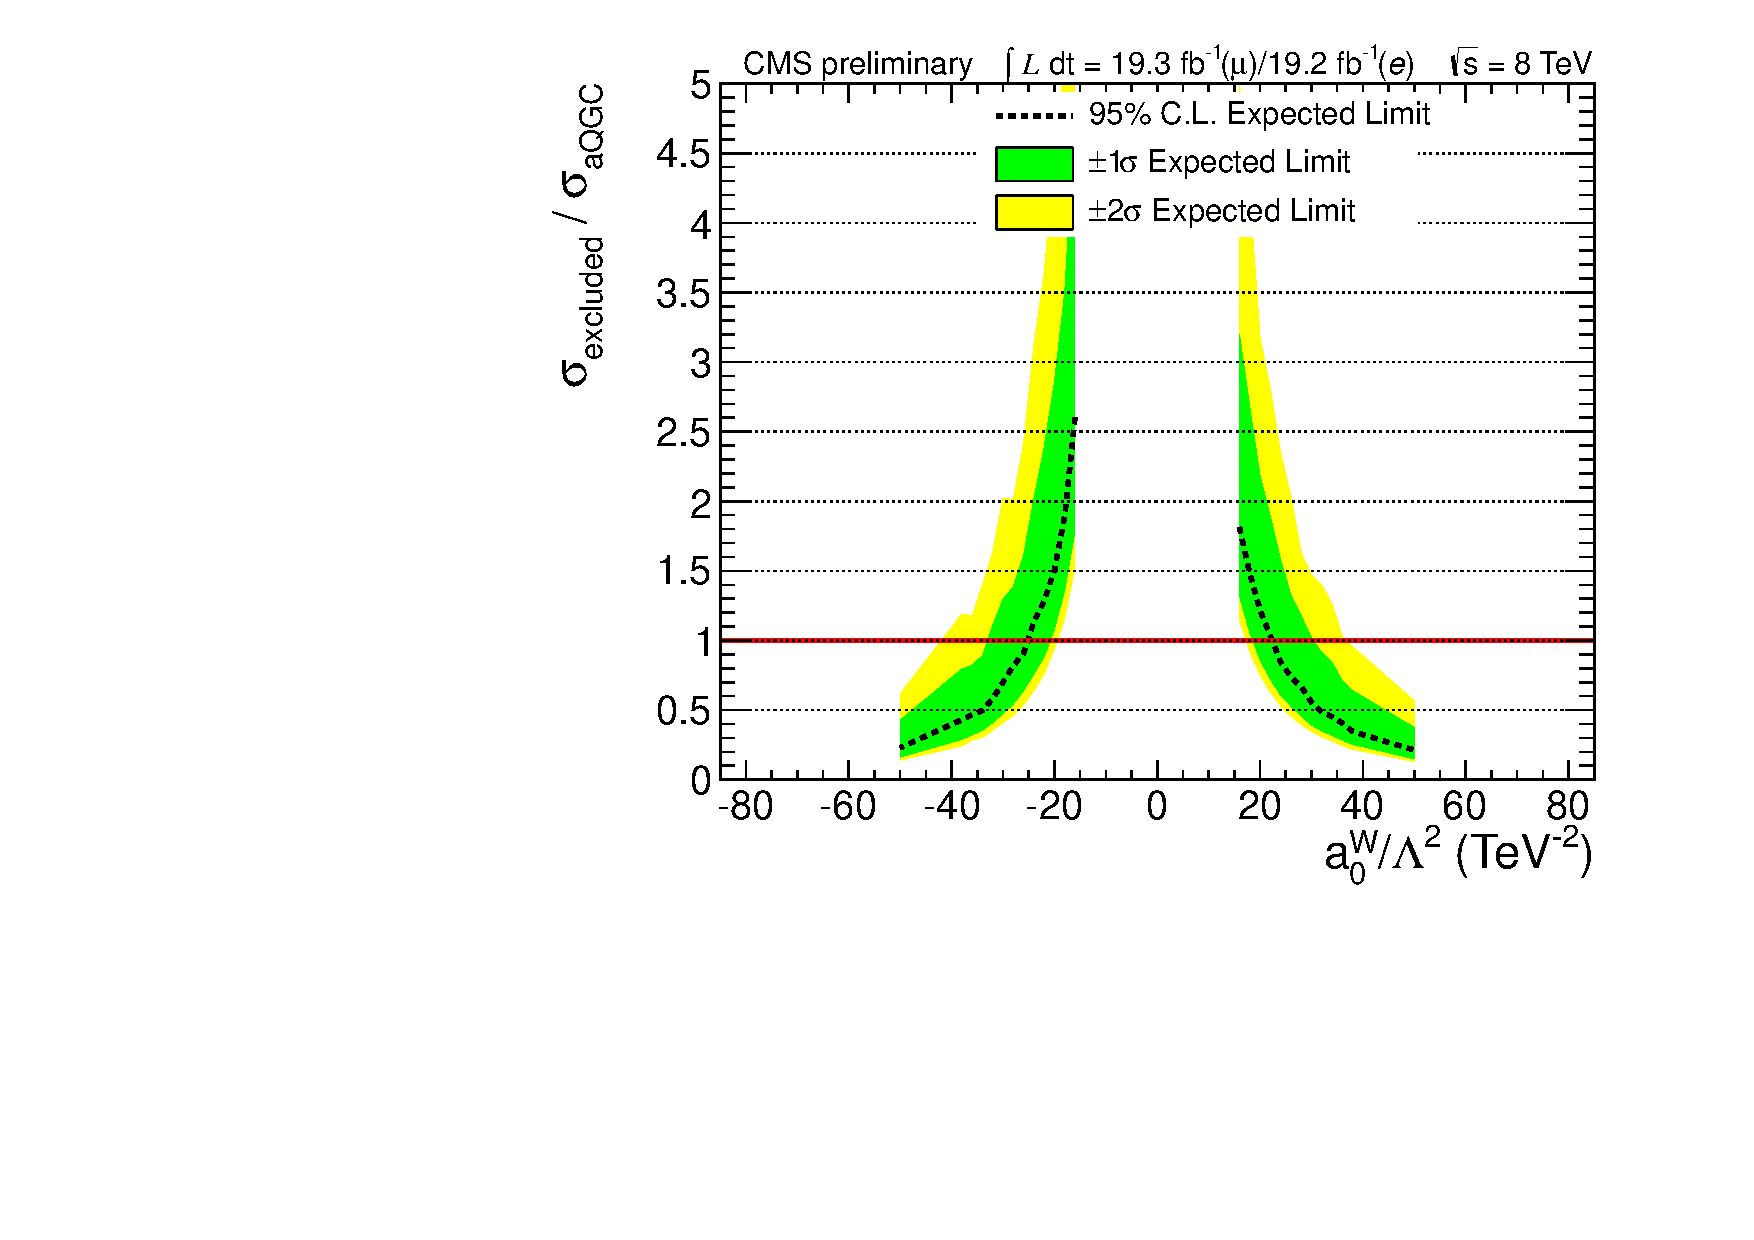
\includegraphics[width=0.33\textwidth]{figs/a0W_PhotonPT_limit_MVA02.pdf}
  }
    \subfigure[]{
    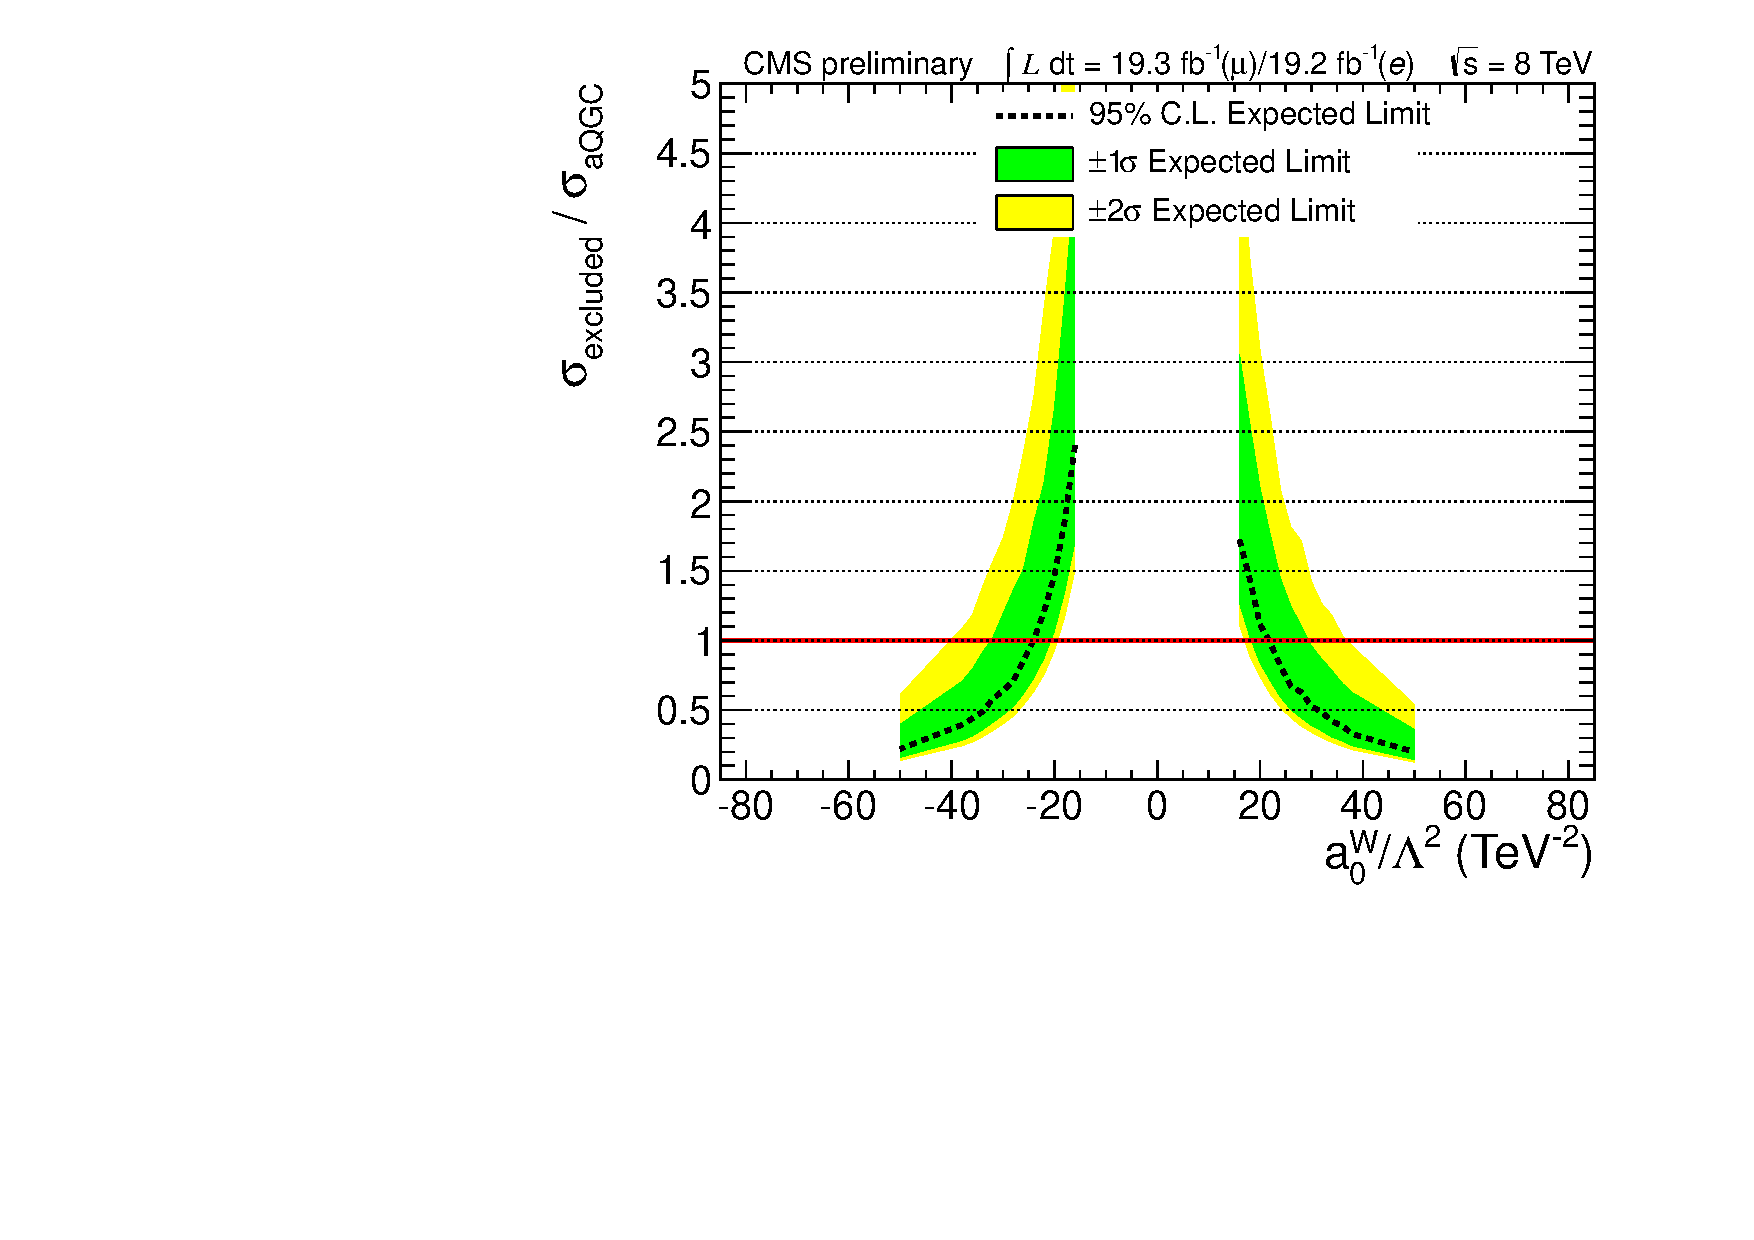
\includegraphics[width=0.33\textwidth]{figs/a0W_PhotonPT_limit_MVA03.pdf}
  }\\
    \subfigure[]{
    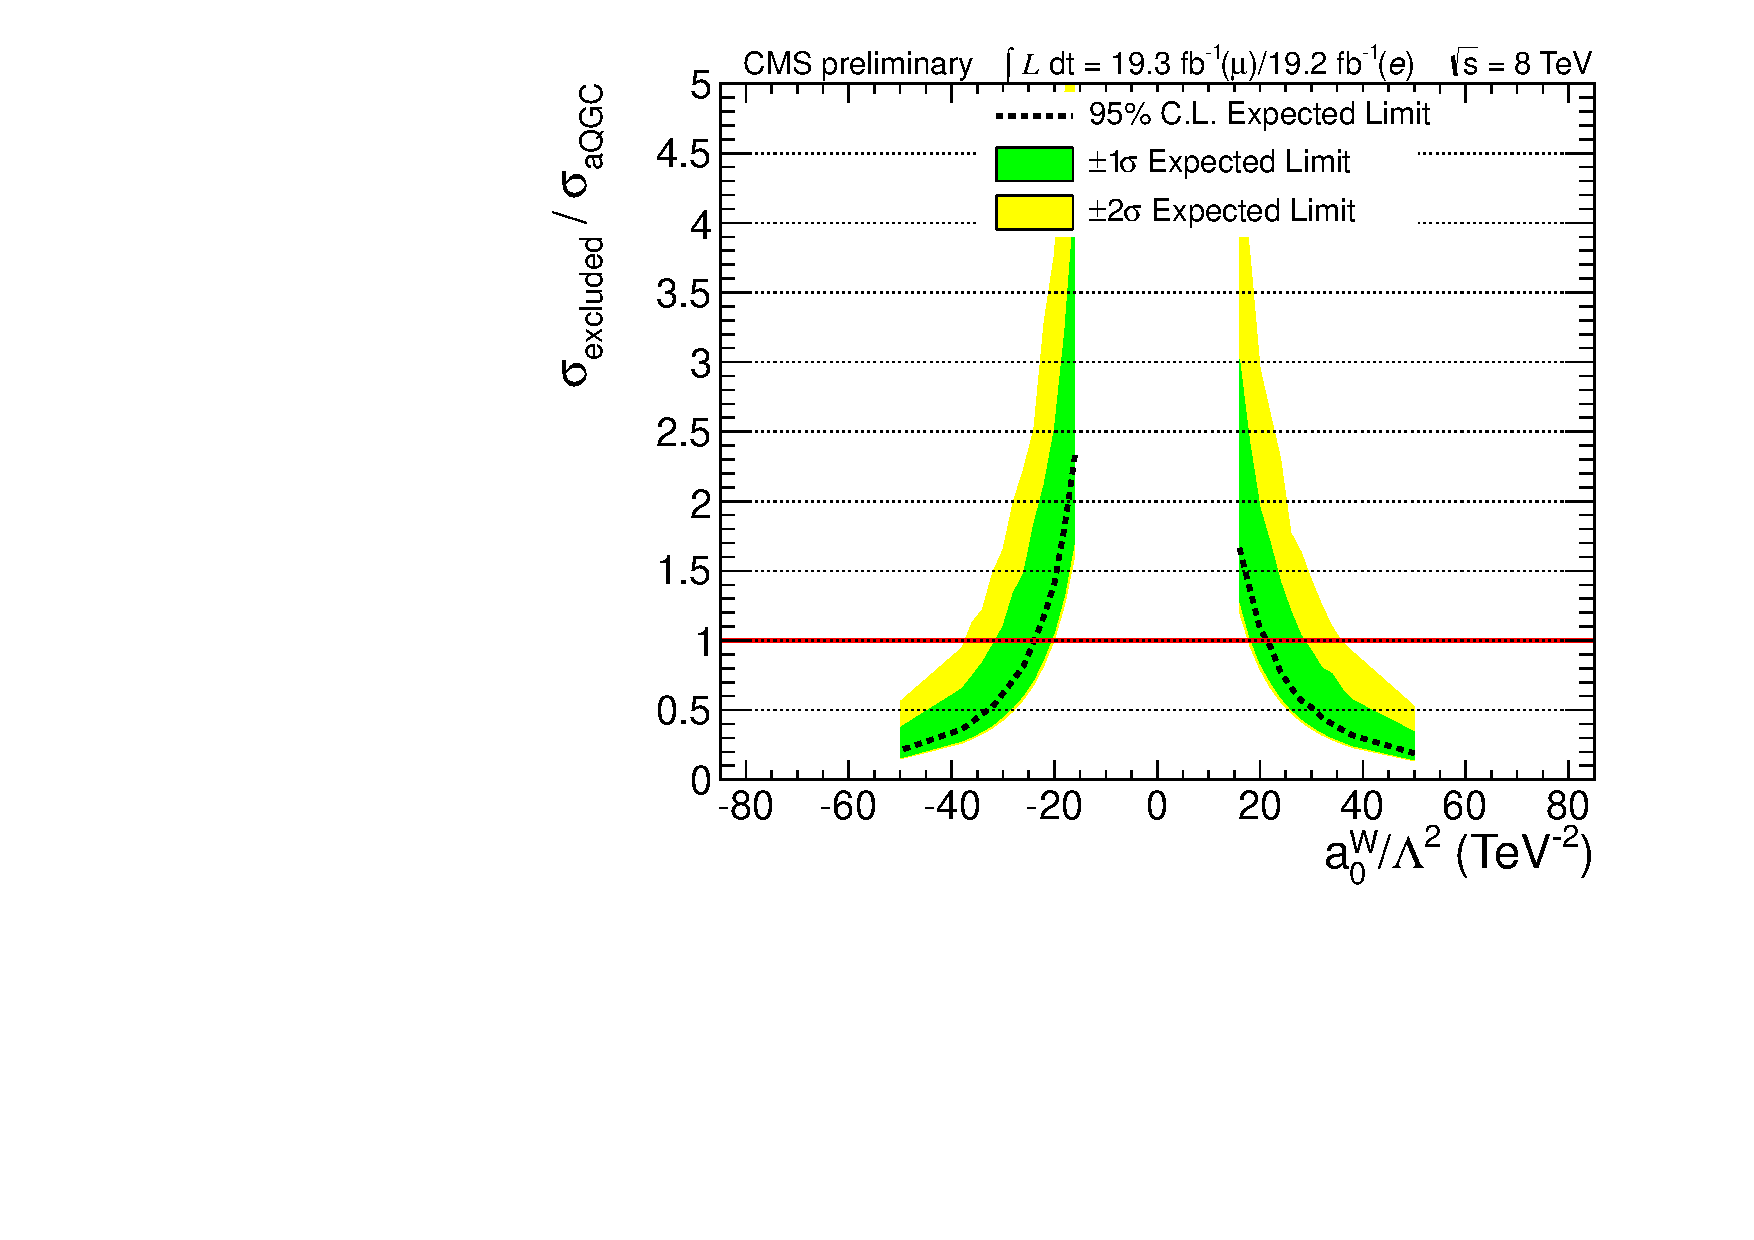
\includegraphics[width=0.33\textwidth]{figs/a0W_PhotonPT_limit_MVA04.pdf}
  }
    \subfigure[]{
    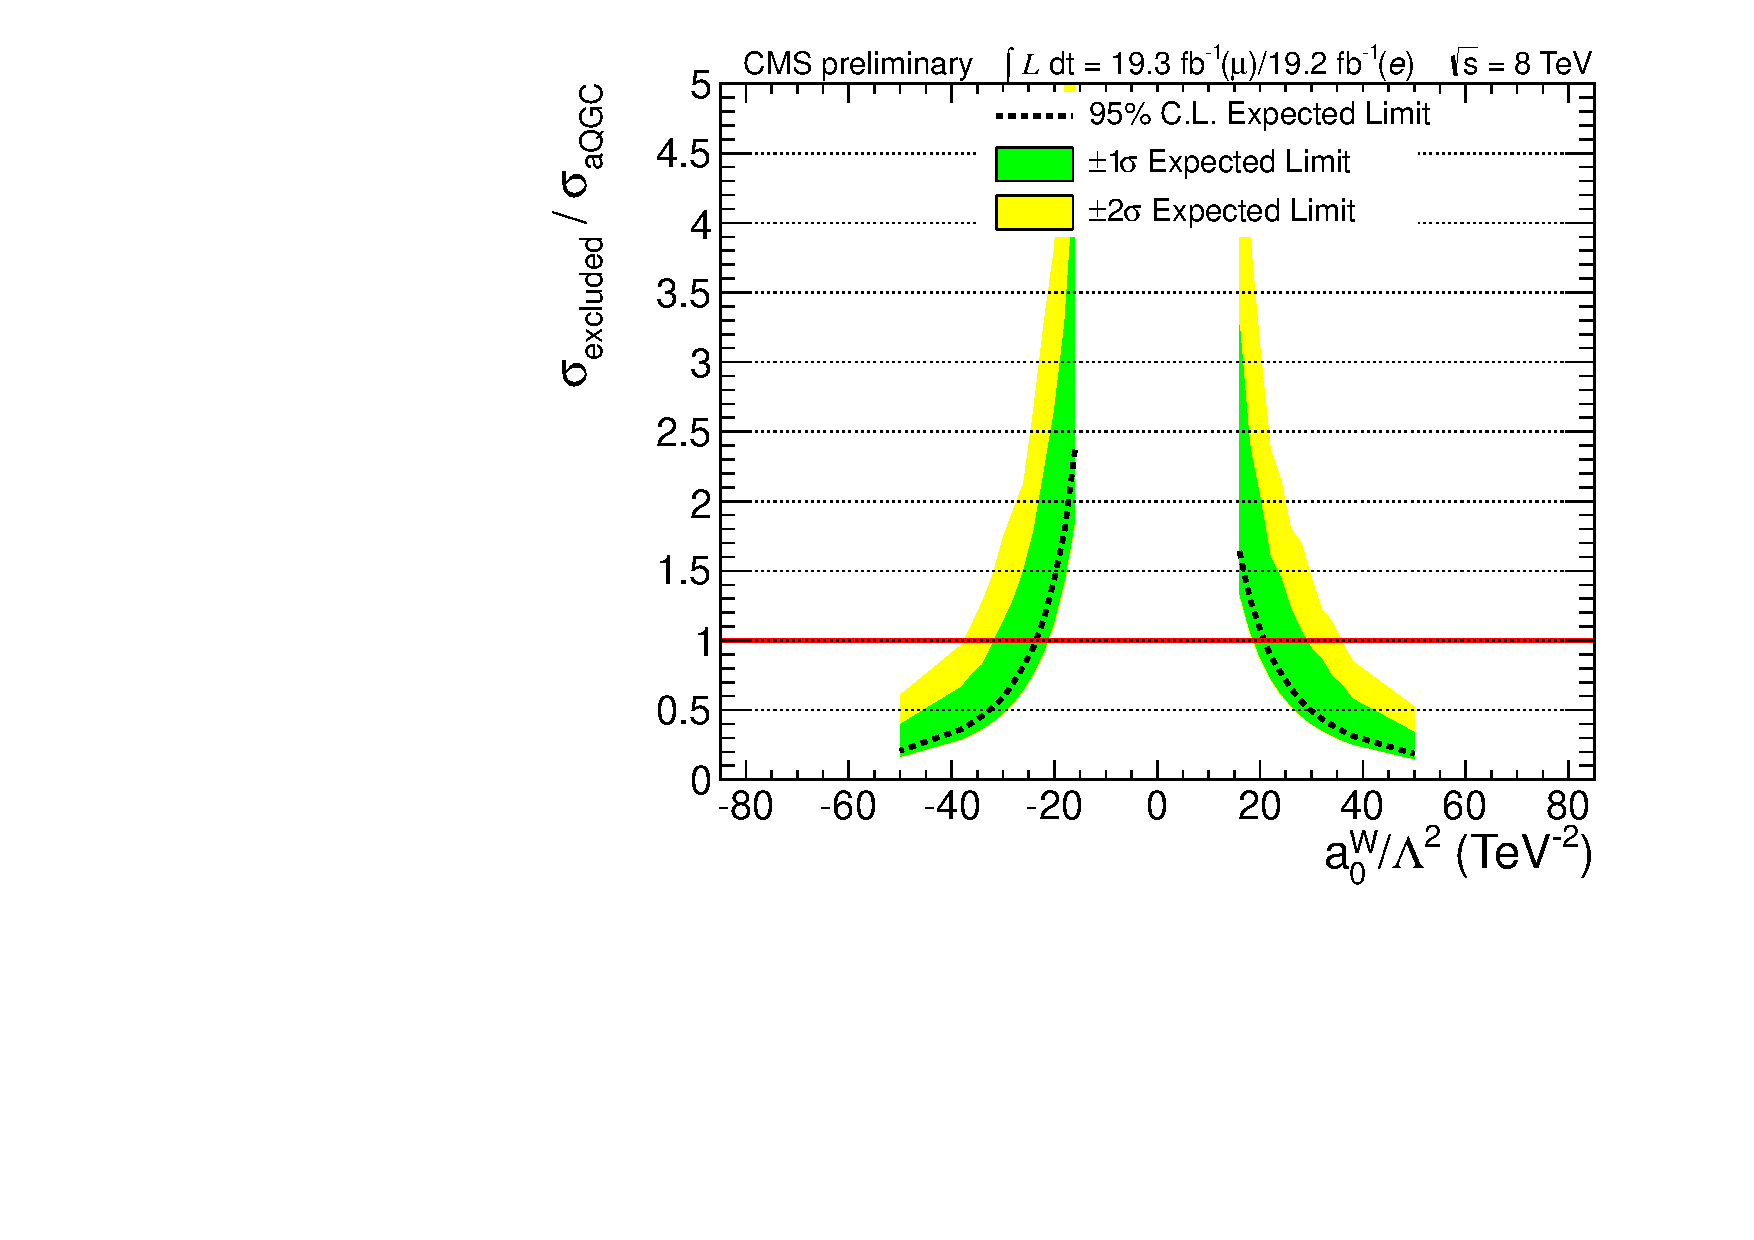
\includegraphics[width=0.33\textwidth]{figs/a0W_PhotonPT_limit_MVA05.pdf}
  }
    \caption{ Exclusion limits for $a_{0}^{W}/\Lambda^{2}$ at 95\% CL and MVA optimization cut at: (a) 0.1, (b) 0.2, (c) 0.3, (d) 0.4, and (e) 0.5, using Photon $p_{T}$.}
    \label{fig:limits_MVA}
  \end{center}
\end{figure}

\begin{figure}[hb]
  \begin{center}
    \subfigure[]{
    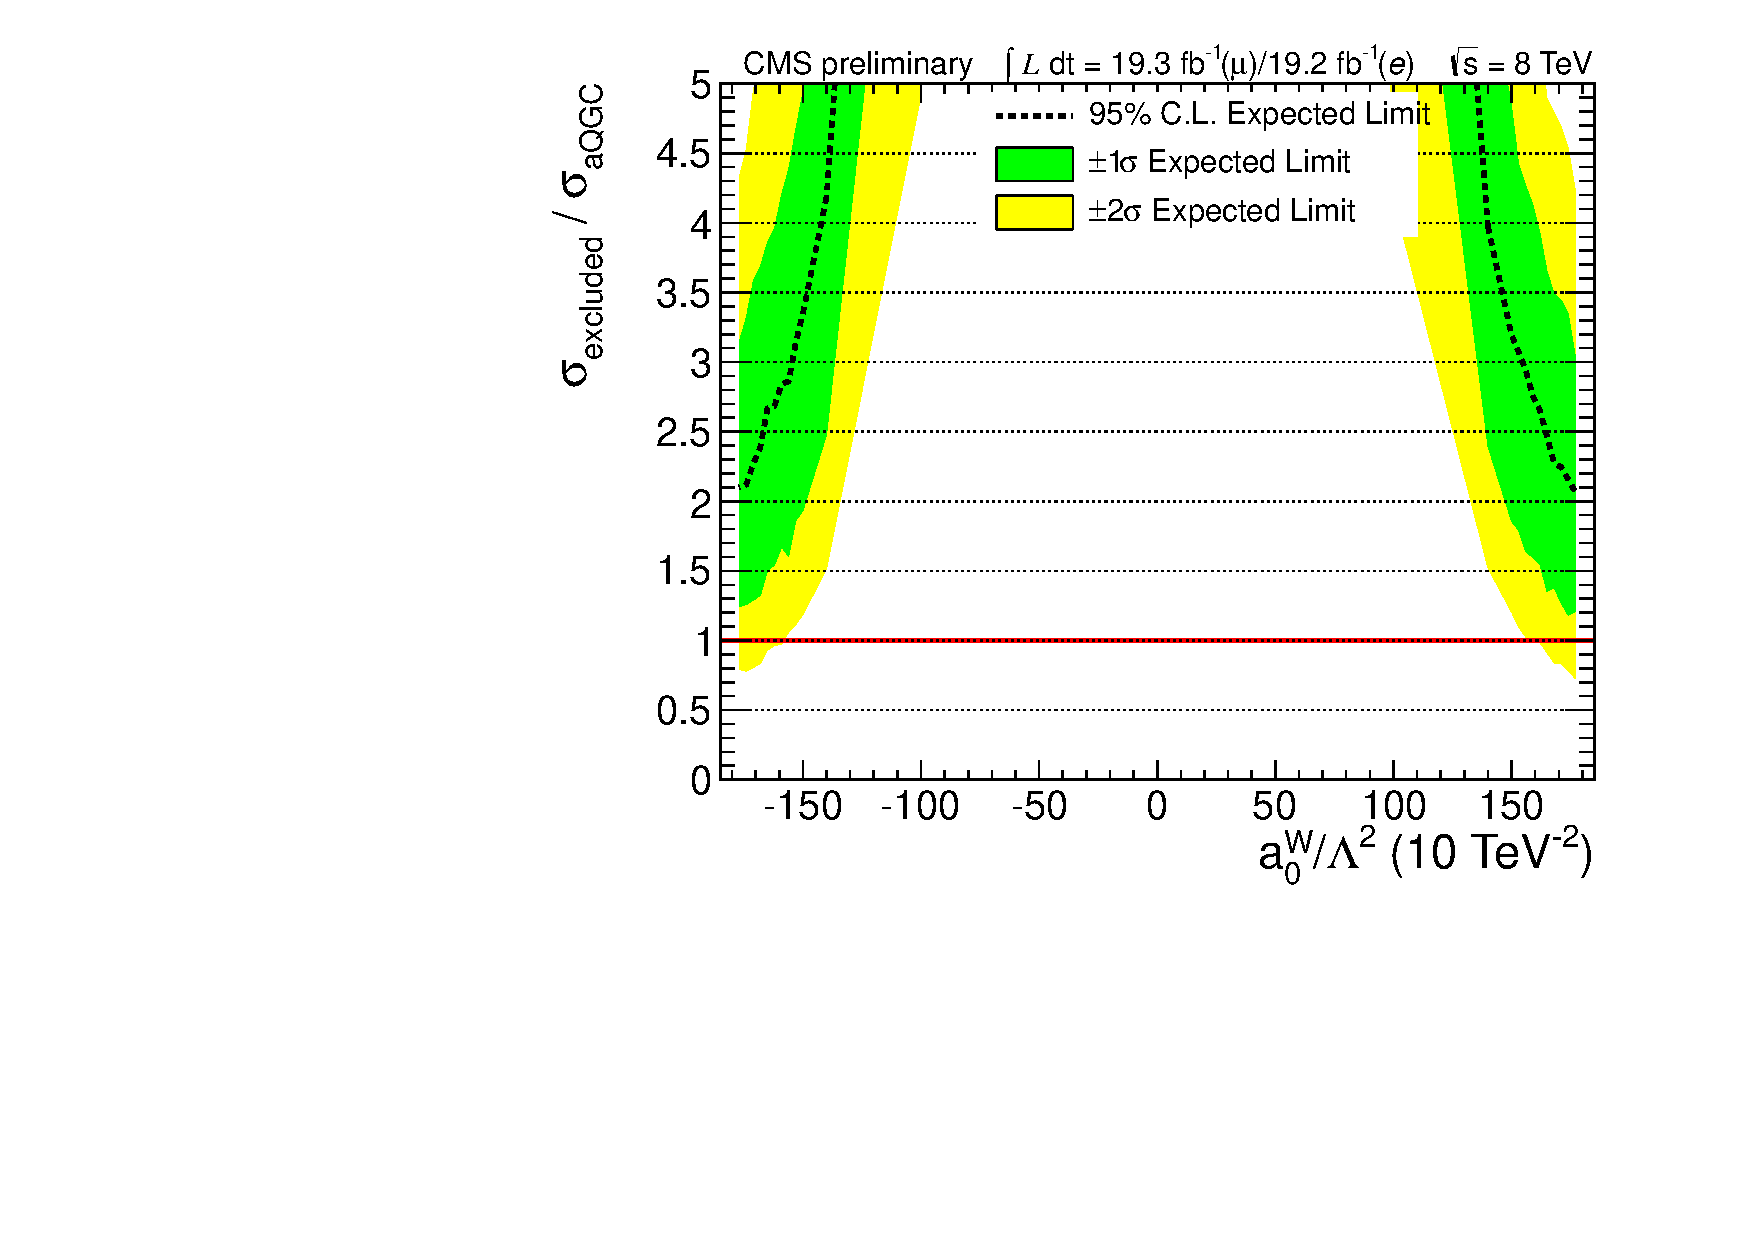
\includegraphics[width=0.33\textwidth]{figs/a0W_PhotonPT_limit_MVA01_500FFn2.pdf}
  }
    \subfigure[]{
    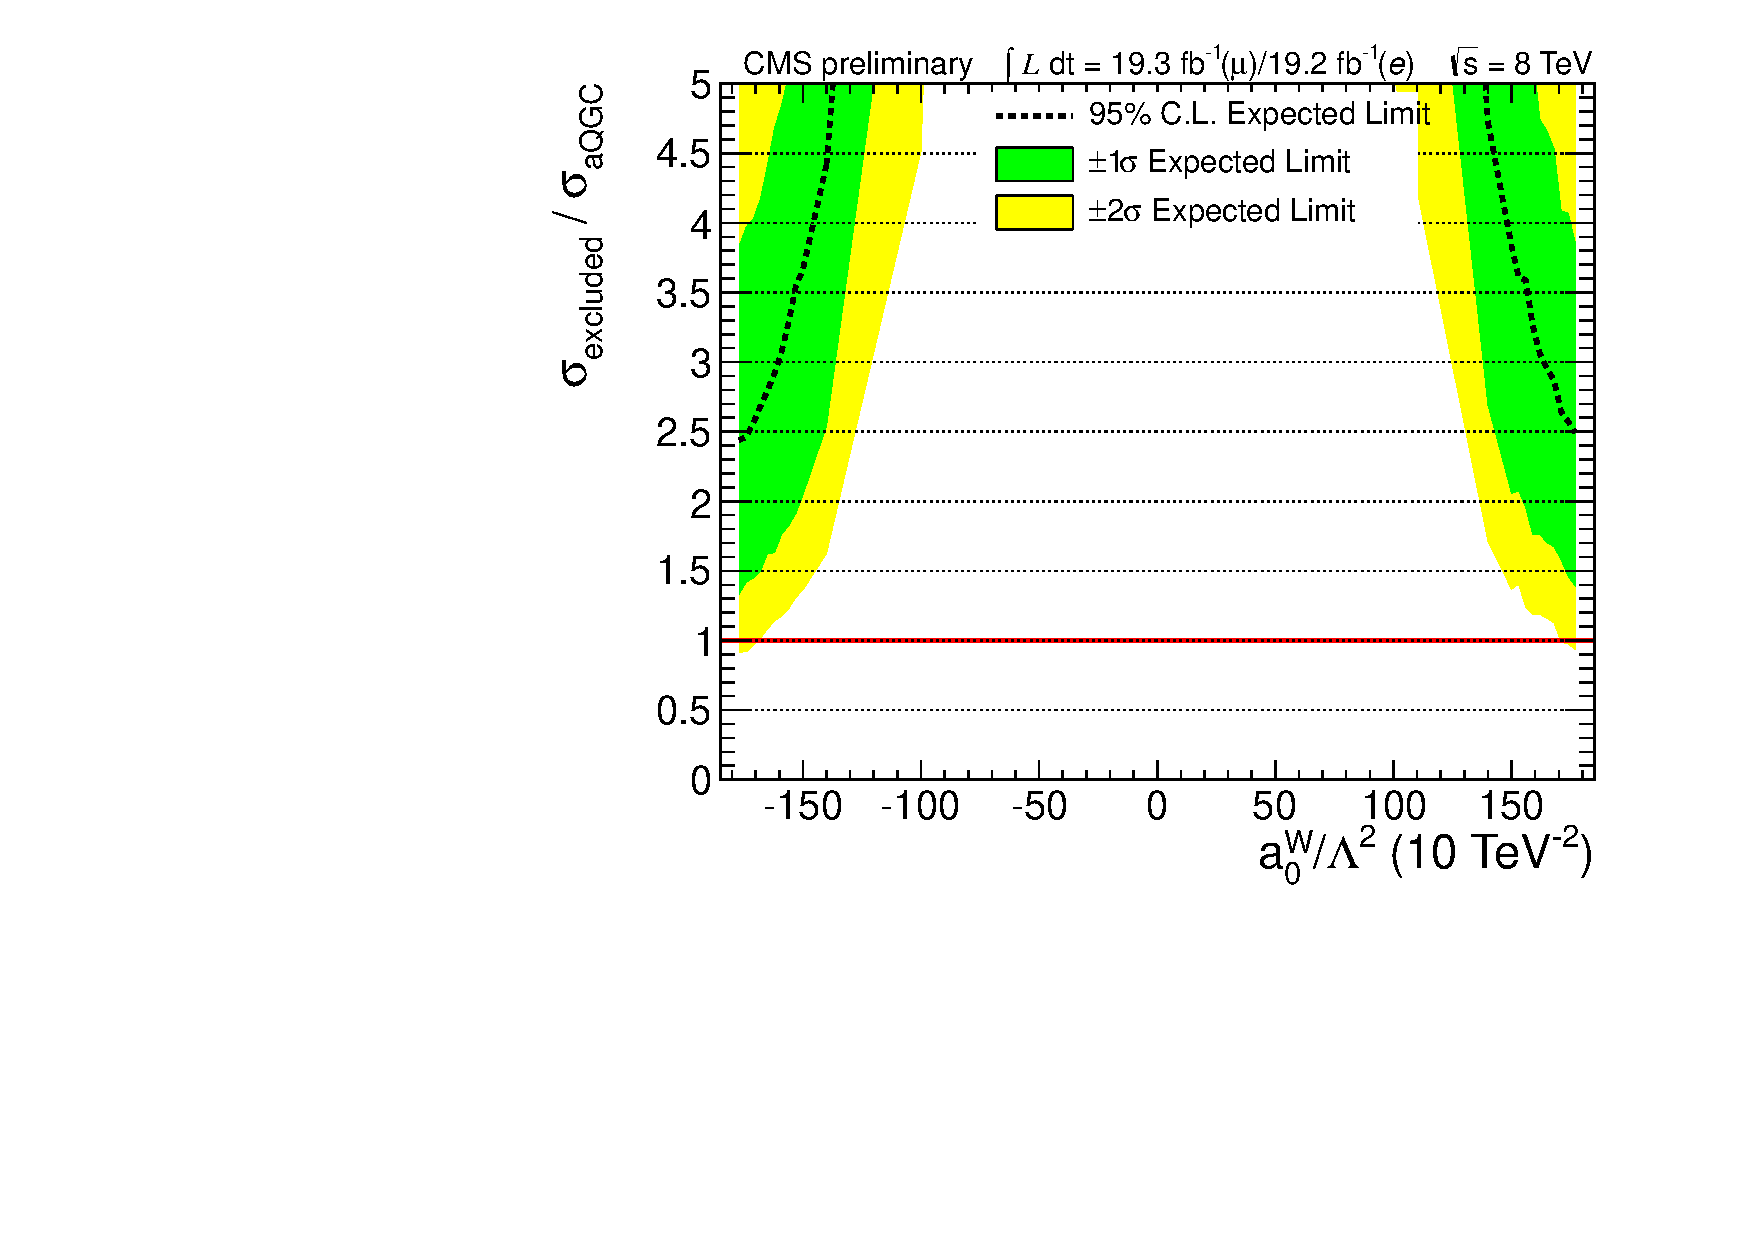
\includegraphics[width=0.33\textwidth]{figs/a0W_PhotonPT_limit_MVA02_500FFn2.pdf}
  }
    \subfigure[]{
    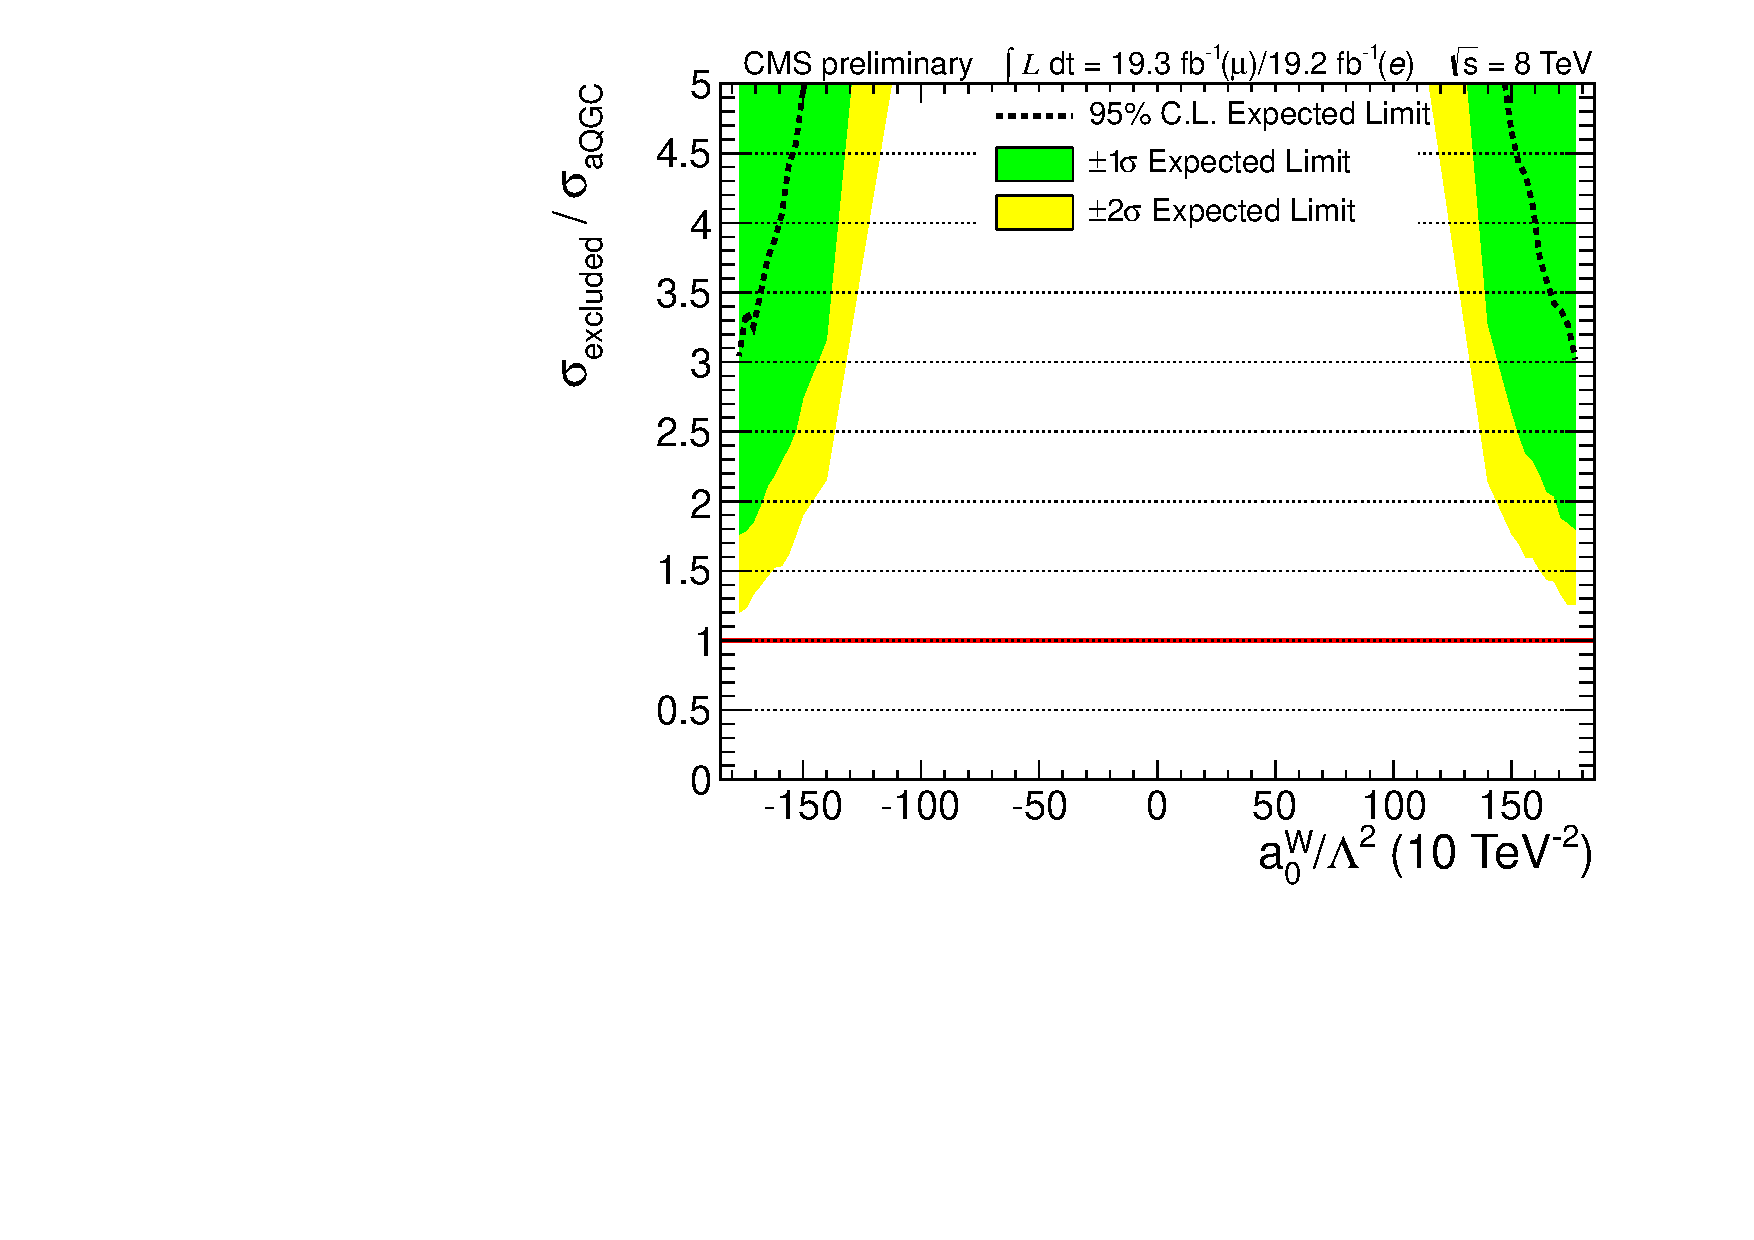
\includegraphics[width=0.33\textwidth]{figs/a0W_PhotonPT_limit_MVA03_500FFn2.pdf}
  }
    \caption{ Exclusion limits for $a_{0}^{W}/\Lambda^{2}$ at 95\% CL and MVA optimization cut at: (a) 0.1, (b) 0.2, and (c) 0.3 using Photon $p_{T}$ and Form Factor $\Lambda = 500 GeV, n = 2$.}
    \label{fig:limits_MVA_FF}
  \end{center}
\end{figure}

\subsection{$a_{0}^{W}$ Limits using Photon $p_{T}$-dependent K-Factor}
\label{sec:limits_pTKFact}
In order to verify that our limit setting procedure is not neglecting
possible new physics, we produced a photon $p_{T}$-dependent K-factor
for the parameter $a_{0}^{W}$. Our procedure outlined in 
Section~\ref{sec:aQGC_Kfac} applys a constant Drell-Yan like K-factor
of 1.185 to the resulting spectrum after removing the SM prediction 
of the signal; the limits shown in Figure~\ref{fig:limits_functKfac} are derived
by first applying a AQGC-and-photon-$p_{T}$-dependent K-factor
to the predicted AQGC sample and then removing the SM prediction that
has had its SM 2.1 K-factor applied. 
Figure~\ref{fig:limits_functKfac} and Table~\ref{tab:limit_values_funcKFac}
demonstrate that the effect is minimal.

\begin{table}[htb]
\centering
\scalebox{1.0}{
  \begin{tabular}{|c|c|}
  \hline
  Observed Limits & Expected Limits \\
  \hline
  \hline
  -24 ($TeV^{-2}$) $<$ $a_{0}^{W}/\Lambda^{2}$ $<$ 20 ($TeV^{-2}$)  & -27 ($TeV^{-2}$) $<$ $a_{0}^{W}/\Lambda^{2}$ $<$ 22 ($TeV^{-2}$) \\
  \hline
  \end{tabular}}
  \caption{95\% CL shape-based exclusion limits listed for both the muon and electron channels of the AQGC parameter $a_{0}^{W}/\Lambda^{2}$, using photon $p_{T}$, without MVA optimization, and with a $p_{T}$-dependent K-factor.}
  \label{tab:limit_values_funcKFac}
\end{table}

\begin{figure}[hb]
  \begin{center}
    \subfigure[]{
    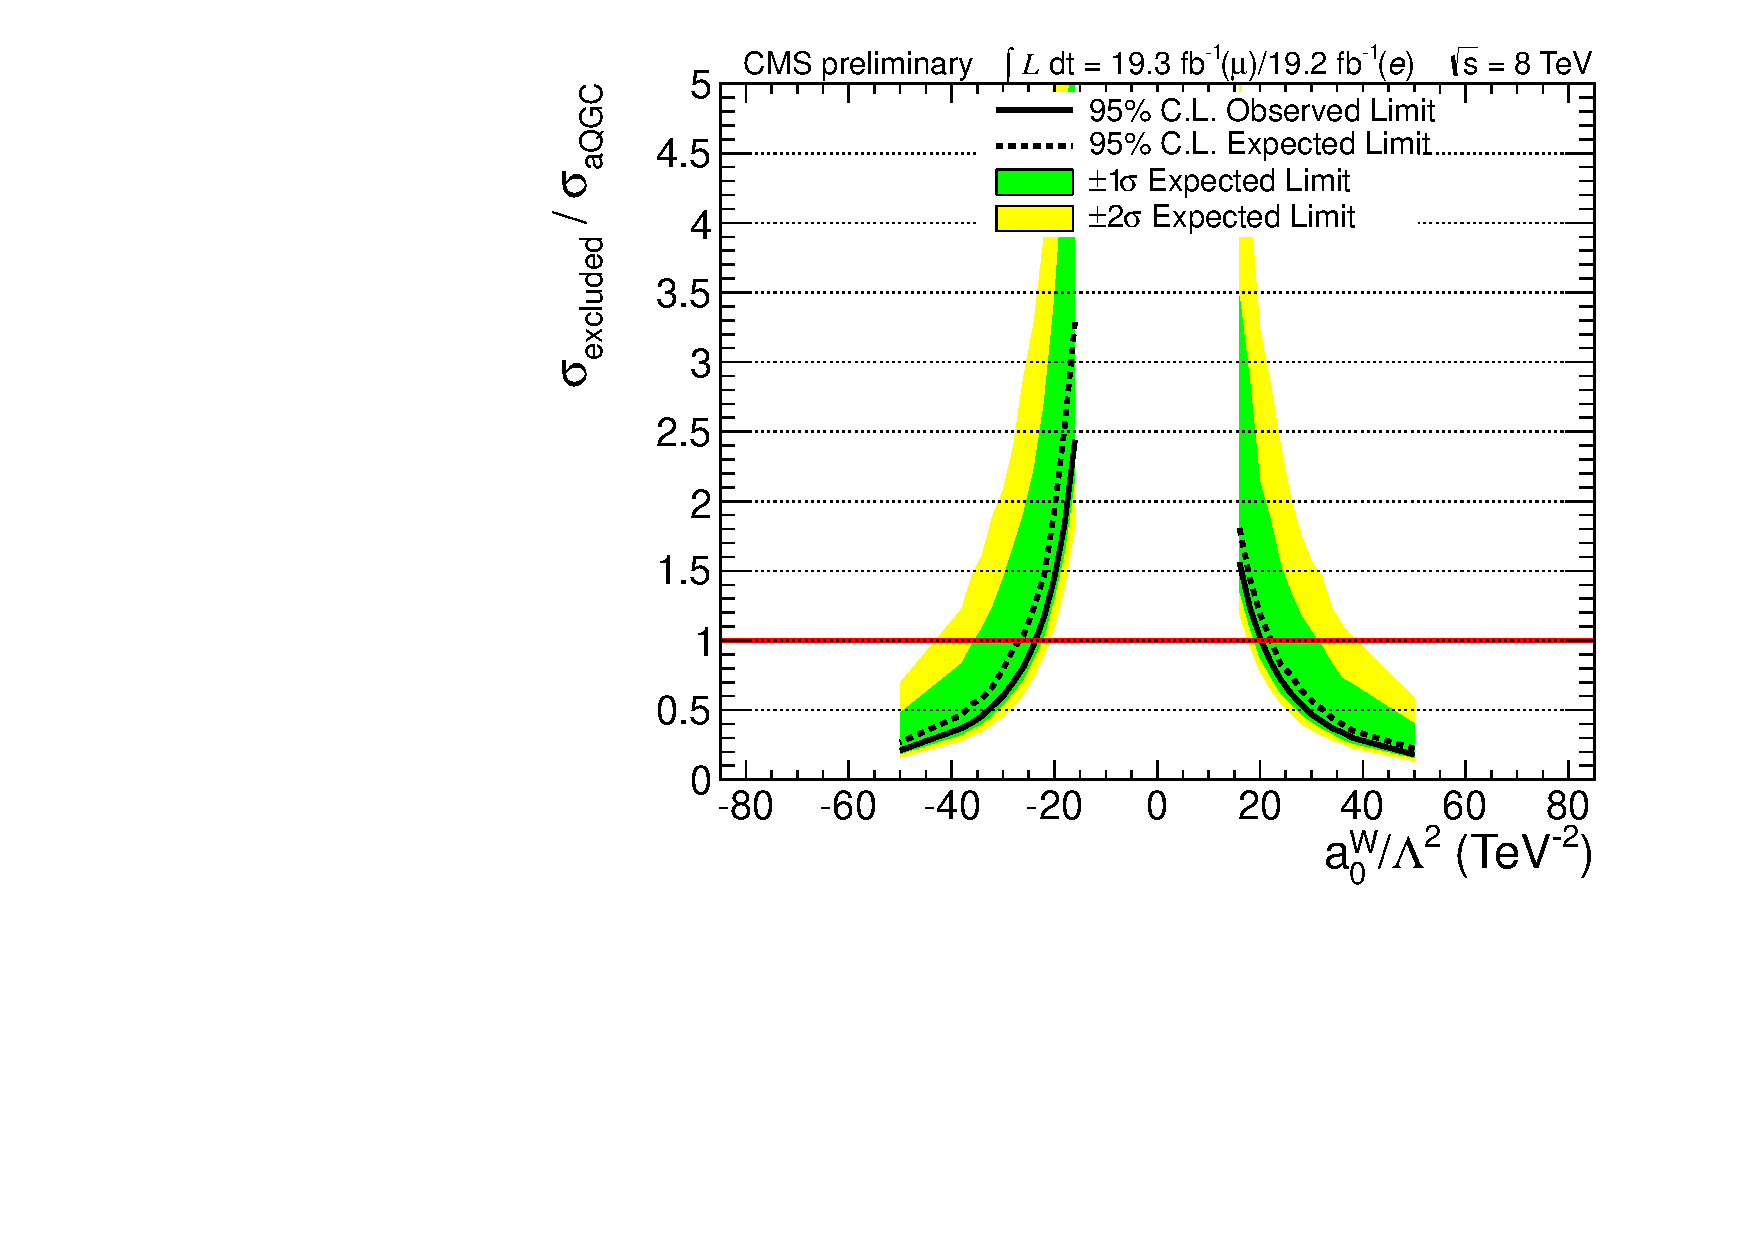
\includegraphics[width=0.45\textwidth]{figs/a0W_PhotonPT_limit_noMVA_functKFac.pdf}
  }
    \caption{ Exclusion limits for $a_{0}^{W}/\Lambda^{2}$ at 95\% CL using photon $p_{T}$-dependent functional K-factors.}
    \label{fig:limits_functKfac}
  \end{center}
\end{figure}

\subsection{$a_{0}^{W}$ Limits using $\Lambda = 500 GeV, n = 2$ Form Factor}
In the investigation of unitarity violation, we have also set limits on
$a_{0}^{W}/\Lambda^{2}$ using a form factor of $\Lambda = 500 GeV and n = 2$.
The limits without MVA optimization are shown in Figure~\ref{fig:limitshape1d_noMVA},
with their values listed in Table~\ref{tab:limit_values_noMVA_FF}. Limits with 
various MVA cuts are shown in Figure~\ref{fig:limits_MVA_FF}.

\begin{table}[htb]
\centering
\scalebox{1.0}{
  \begin{tabular}{|c|c|}
  \hline
  Observed Limits & Expected Limits \\
  \hline
  \hline
  -1480 ($TeV^{-2}$) $<$ $a_{0}^{W}/\Lambda^{2}$ $<$ 1500 ($TeV^{-2}$)  & -1530 ($TeV^{-2}$) $<$ $a_{0}^{W}/\Lambda^{2}$ $<$ 1530 ($TeV^{-2}$) \\
  -5782 ($TeV^{-4}$) $<$ $f_{M,0}/\Lambda^{4}$ $<$ 5705 ($TeV^{-4}$)  & -5898 ($TeV^{-4}$) $<$ $f_{M,0}/\Lambda^{4}$ $<$ 5898 ($TeV^{-4}$) \\
  -2891 ($TeV^{-4}$) $<$ $f_{M,2}/\Lambda^{4}$ $<$ 2853 ($TeV^{-4}$)  & -2949 ($TeV^{-4}$) $<$ $f_{M,2}/\Lambda^{4}$ $<$ 2949 ($TeV^{-4}$) \\
  \hline
  \end{tabular}}
  \caption{95\% CL shape-based exclusion limits listed for both the muon and electron channels of each AQGC parameter $a_{0}^{W}/\Lambda^{2}$, with a Form Factor of $\Lambda = 500 GeV, n = 2$, using photon $p_{T}$ and without MVA optimization.}
  \label{tab:limit_values_noMVA_FF}
\end{table}
